\documentclass[../ala_hataile.tex]{subfiles}
\begin{document}
\twocolumn[\section{Kaupunki nimeltä Helsinki} {\small \itshape ``Helsingissä voi tapahtua aivan mitä vain. Näin voi käydä muissakin kaupungeissa, mutta Helsingissä se tapahtuu useammin. Eilen illalla kävellessäni eduskuntatalon ohi ihmettelin väenpaljoutta. Siellä oli enemmän ihmisiä kuin yhdessäkään samalla paikalla pidetyssä mielenosoituksessa, eikä kysymyksessä nytkään ollut mielensoitus, vaan Kansallisbaletin ilmainen esitys kulttuurinnälkäisille helsinkiläisille.''}\vspace{0.5cm}]
Tervetuloa Helsinkiin! Tarkoitukseni on
esitellä tämän opiskelukaupunkisi resursseja,
ei listata joukkoa itsestäänselvyyksiä.
Muualta tulleille tässä on toivottavasti
kosolti
hyödyllistä tietoa, mutta uskoisin, etteivät
kaikki paikkakuntalaisetkaan
tiedosta
kotikaupunkinsa kaikkia
mahdollisuuksia.
Jokunen sana myös opiskelusta.
\subsection*{Opiskelu?}
Tilanne on monen opiskelijan kohdalla
se, että he ovat pöllähtäneet yliopistoon
joko suoraan koulun penkiltä tai mahdollisesti sotaväestä, eivätkä edes oikein tiedä
miksi täällä ovat. Tämä on kovin yleistä
juuri ML-tiedekunnan kohdalla, koska
sinne hyväksytään suurin osa opiskelijoista
ilman
pääsykoehelvettiä. Ei kuitenkaan
kannata
jäädä tumput taskussa seisomaan,
vaan siitä vain opiskelemaan ja katsomaan
mikä kiinnostaa vai kiinnostaako mikään.
Jos sen aineen, johon sinut hyväksyttiin,
opinnot
eivät maistu, voit aika vapaasti
opiskella
lähes kaikkia yliopistossa opetettavia
aineita, ainakin ensimmäisten vuosien
opintoja.

Ja vaikka se oikea ala ei heti löytyisikään, ei kannata masentua, sillä on parempi tehdä
jotain sellaista, mikä kiinnostaa,
kuin valmistua
jostain aineesta periaatteella
``kun
nyt ei oikein mitään muutakaan
ollut'' ja
sitten vielä työskennellä loppuikä samalla
alalla. Tämä tosin yleensä
vältetään, sillä
korkeakoulututkinto on kuitenkin sen verran
``kova juttu'', että sen läpivieminen vaatii
kyllä kiinnostusta asiaan.
\subsection*{Solu = cell = selli}
Pääkaupunkiseudulla on opiskelija-asunnoista
syksyisin kova pula, joten etenkin
Uudellamaalla asuvat saattavat joutua
odottamaan asuntoa HOAS:lta tai ylioppilaskunnalta
pitkälle talveen ja junailemaan
ensimmäisen syksyn. Opiskelijasolujen
vuokrataso ei ole kuitenkaan kovin korkea,
ja osakuntien opiskelija-asunnot
ovat maan
edullisimpia.
\begin{figure*}[h!]
	\centering
	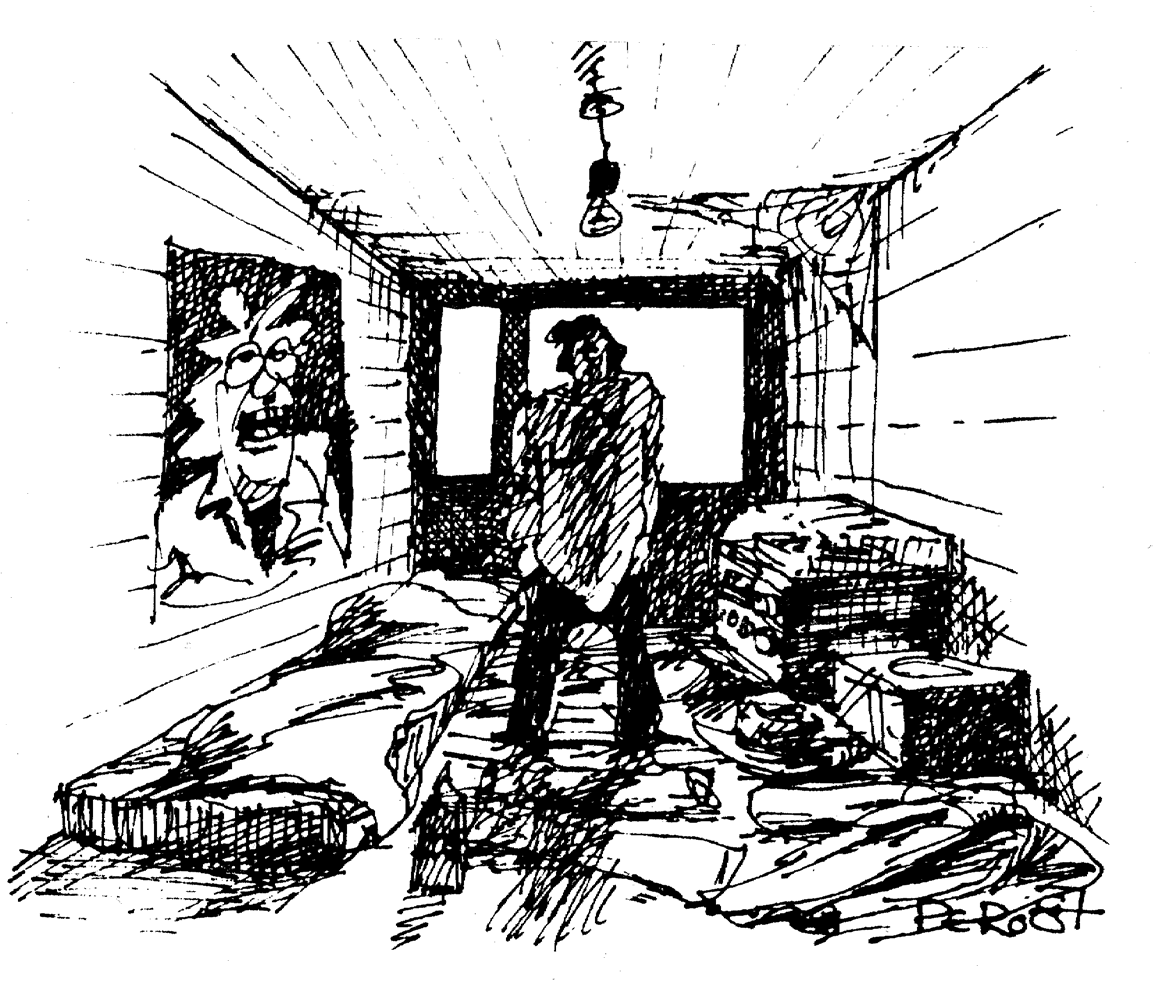
\includegraphics[width=0.8\textwidth]{soluasunto.png}
\end{figure*}

Jos on kipeästi asunnon tarpeessa, niin
ainakin HOASille kannattaa jättää hakemus
ja sitten soitella aktiivisesti. Voi myös
käydä katsomassa nettisivuilta juuri vapautuneita
paikkoja.

Vapaat markkinat tarjoavat hintavan
vaihtoehdon, vaikka vuokrat eivät ole
nousseet merkittävästi viime vuosina.
Jos kuitenkin onnistuu saamaan isomman
kaveriporukan kasaan ja onni on myötä,
saattaa löytää itsensä asumasta hienosta
asunnosta läheltä keskustaa siedettävään
hintaan.
\subsection*{Elämä}
Ajatus tuskin sinua edes kiinnostaa,
mutta on koko lailla mahdotonta käyttää
kaikkea aikaa opiskeluun. Mukava yhteensattuma
puolestaan on se, että Helsinki
tarjoaa sinulle mitä parhaimmat mahdollisuudet
tehdä mitä tahansa. Täällä voit vapautuneesti harjoittaa juuri sitä mitä haluat,
tarjontaa löytyy kaikissa harrastuksissa
ja
aktiviteeteissä, ja niissä kohtaat varmasti
samanhenkisiä ihmisiä.

Eikä Helsinki pure, vaikka jonkun mielestä
saattaa aluksi vähän murista. Silti
joku sulkee silmänsä ja ``tuhlaa'' elämäänsä
ja rahojaan matkustamalla joka ikinen viikonloppu
takaisin kotipuoleen, mutta suurin
osa sisäistää ajatuksen ``tärkeintä on se
missä on, ei se missä ei ole''.

Ja kun siltä alkaa tuntua, niin Helsingin
``kansalaisuuden'' saat nopeasti vierailemalla
maistraatissa Albertinkadulla tai
muutaman arkipäivän viiveellä esimerkiksi
Nettipostin osoitteenmuutoksen kautta.
Samalla aukeavat
taivaan portit mm.~mahdollisuuteen
äänestää ja vaikuttaa siellä
missä asuu, sekä muut etuudet, varsinkin
hesalaisten mahdollisuus
liikennelaitoksen
edullisempiin piletteihin.
\subsection*{Leffaviikko}
Jos Limeksen elokuvakerho LiEKe ei
pysty ilmaisilla näytöksillään tukahduttamaan
elävän kuvan himoasi, on edessäsi
Helsingin leffatarjontaan tutustuminen. Ja
sitähän riittää.

Helsingistä löytyy kaksi suurta elokuvakeidasta,
Kaisaniemen Kinopalatsi (10~salia) ja Kampin Tennispalatsi (14~salia).
Niiden lisäksi kaupungissa on kymmenisen
muuta Finnkinon, Cinema Mondon ja
pienempien alan yritysten teatteria. Elokuva-arkistoakaan ei tule unohtaa, siellä
esitetään vuosittain satoja vanhoja ja uusia
klassikkoja edulliseen hintaan. Monen eri
ketjun sarjalippujen ostaminen saattaa olla
hintavaa, joten kannattaa yrittää bongata
järjestöjen leffaexcuja ja "-iltoja tai järjestää
sellainen itse.

Syksyisin Helsingissä vietetään Rakkautta
\& Anarkiaa "-festivaalia, jonka
mielenkiintoiseen ohjelmistoon kannattaa
tutustua ajoissa etukäteen ja hankkia liput
heti niiden tullessa myyntiin. Helsingissä
järjestetään myös lukuisia muita elokuvatapahtumia,
kuten outojen elokuvien yölliset
Night Visions "-festarit sekä suomalaista
lyhyt\-elokuvaa esittelevä Helsingin lyhyt\-elokuva\-festivaalit
(entiseltä nimeltään Kettupäivät).
\subsection*{Musiikkia korville}
Vilkaisu esimerkiksi Helsingin uutiset
"-lehden menopalstalle saa varmasti vakuuttumaan:
tästä kylästä ei musiikki lopu. Eikä
pelkästään rokkenrollia tai teknojumputusta,
vaan alle kympillä voi istua uudessa
lasisessa Musiikkitalon kuutiossa kuuntelemassa
esim.\,Helsingin kaupungin\-orkesteria tai Radion sinfoniaorkesteria. Myös oopperaan kannattaa käydä tutustumassa
opiskeluaikana, kun liput eivät vielä maksa
maltaita.

Ulkomaanihmeet ja kotimaiset kuuluisuudet
poikkeavat myös säännöllisesti
kaupungissa, kuka Tavastialla tai Vanhalla,
kuka Hartwall Areenalla. Eksoottisempaa
musiikkia tarjoavat puolestaan täällä asuvat
ulkomaalaiset omissa ravintoloissaan ja
klubeissaan.
\begin{figure*}[!b]
	\centering
	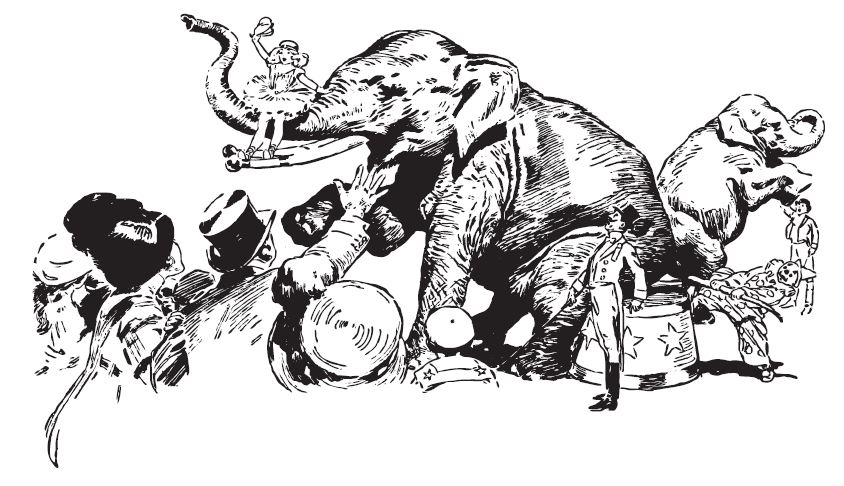
\includegraphics[width=\textwidth]{norsut.jpg}
\end{figure*}
\subsection*{Ryhmä teatteriin}
Kansallisteatteri, Kaupungin\-teatteri,
KOM-teatteri, Q-teatteri, Ryhmä\-teatteri,
Studio Pasila, Yli\-oppilas\-teatteri, Teatteri\-korkea\-koulu.
Lukematon määrä suuria ja
pieniä esityksiä pyörii ja pyörittää ympäri
vuoden. Kesäisin mm.\,Suomenlinnassa
esitetään
kesäteatteria. Jälleen opiskelija
saa alennusta, joten kannattaa tutustua
teatteritaiteeseen.
Teatterista, oopperasta,
konserteista
ym.\,kiinnostuneiden kannattaa
seurata Limeksen sähköpostilistan ilmoituksia
kulttuuriexcuista.
\subsection*{Ruumiin kulttuuri}
Muidenkin ruumiinosien kuin baarioppaan
avulla keskivartalon rakentamisesta
kiinnostuneiden on parasta ensin tutustua
UniSportin tarjontaan ja Limeksen liikuntatoimintaan,
ja sännätä vasta sitten
kalliimmille punttisaleille, joita niitäkin
on kaupunki pullollaan. Ja mitä eksoottisimmillekin
urheilulajeille löytyy oma
seura! Jo oman opiskelutehonkin ylläpitämiseksi
kannattaa liikkua -- kipeiden niskojen
takia YTHS:llä juokseminen on lopulta
paljon tylsempää. Kumpulan liikuntakeskus
tarjoaa myös paljon erilaisia ohjattuja
tunteja kaikilla tasoilla. Näillä jaksaa tulla
vaikkei muuten innostuisikaan raudan
pumppaamisesta
salilla, lisäksi tunneilla
näkee muutakin kuin oman kampuksen porukkaa!

Ja lopuksi: opiskelijan kannattaa kysyä
alennusta. Aina ja kaikesta.

\twocolumn[\section{Jöröillä järsittävää} {\small \itshape ``\dots eli missä opiskelija syö lounaansa?''}\vspace{0.5cm}]
\subsection*{Unikahvilat}
Luonnollisin ratkaisu opiskelijan päivittäisiin
nälkätiloihin löytynee UniCafen
ravintoloista, joita löytyy kampusalueilta
parisenkymmentä. Niissä on mahdollista
syödä parilla eurolla niin paljon kuin vain
jaksaa, ja vieläpä terveellisesti. Päivittäiset
ruokalistat ja tarkat aukioloajat löytyvät kätevästi
netistä \url{www.unicafe.fi}. Kätevämpi
käyttöliittymä ruokalistoihin löytyy osoitteesta
\url{www.varjocafe.net}. Google Playstä löytyvä UniMenu-sovellus tarjoaa opiskelijahintaisten \mbox{UniCafe-}, Amica- ja Sodexo-ravintoloiden ruokalistat kätevästi puhelimeen.

Ravintolat jakaantuvat karkeasti ottaen
kahteen kastiin, keskustan isoihin syöttölöihin
ja osastojen pienempiin kuppiloihin.
Isoimmista eli Pääkkäriltä ja Ylioppilasaukiolta
saa lounasta vielä myöhään iltapäivällä,
kun pienemmissä joutuu jo tyytymään
pelkkään kahviin. Kannattaa myös
huomata, etteivät pienemmät kuppilat
yleensä tee itse ruokiaan, vaan ne tulevat
jonkun isomman ravintolan keittiöstä. Ruokalistat
saattavat siis olla samat eri ravintoloissa.
\begin{figure}[!b]
	\centering
	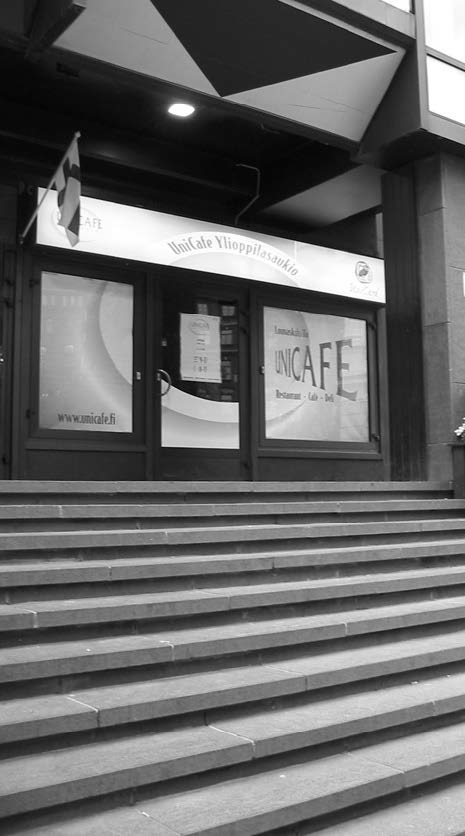
\includegraphics[width=\columnwidth]{yoaukio_unicafe.png}
\end{figure}

Yleisesti ottaen ruoan taso on melko
hyvä -- se vain vaihtelee joskus turhan paljon.
Leipäpöydät ovat yleensä erinomaisia,
eikä salaattivalikoimaakaan voi pitää huonona.
Ruokapöydän jutut muuten vaihtelevat
huomattavasti paikan mukana. Kannattaa
siis pitää korvat auki lounasta syödessä:
saatat esimerkiksi päästä seuraamaan poliittista
debattia Valtsikassa tai filosofien
eksistentiaalista kriisiä Metsätalolla.
\subsection*{Keskustan kuppilat}
\subsubsection*{Pääkkäri}
Valtsikan ohella ainut UniCafe, jossa
on hieno historiallinen ympäristö. Erilaisia
ruokavaihtoehtoja on tavallisina arkipäivinä
runsaasti tarjolla epämääräisistä salaateista
kunnon schnitzeliin. Kotikalja on
todistetusti koko yliopiston parasta. Kumpulan
liemi on tosi pahanmakuista litkua
siihen verrattuna. 

Henkilökunta on ystävällistä
ja palvelualttiimpaa kuin Kaivopihalla
tai Metsätalossa. Lämpimänä vuodenaikana
ruokansa voi nauttia myös ulkosalla,
tunnelmallisella sisäpihalla. Talvella taas
voi katsella ikkunapaikoilta, kuinka räntä
valuu Aleksanterinkadulla spåraa odottavan
harmaan kansan niskaan. Asiakaskunta
koostuu humanisteista, kuten suomenkielen
opiskelijoista, historioitsijoista ja muista pehmeiden tieteiden lukijoista.

Kiihkoateisteille on satunnaisesti tarjolla
jumaluusopillisia väittelyitä. Naapuritalon
teologit käyvät myös usein aterioimassa
täällä.
\subsubsection*{Ylioppilasaukio}
Yksi suurimmista, ellei jopa suurin
UniCafe ydinkeskustassa. Valikoima on
UniCafe-mittapuulla hyvä, salaatteja on
useita erilaisia, kuten pääruokiakin. Kannattaa
tosin varautua erittäin pitkiin jonoihin,
jos tänne eksyy suosituimpiin ruokaaikoihin,
eli puolilta päivin tai noin kahden
maissa. Onneksi tällöin on tosin toinen
linjasto helpottamassa pahimpia ruuhkia.
Huomion arvoista on myös se, että tämä on
ainoa UniCafe, josta saa ruokaa vielä 16.30
jälkeen, sekä lauantaisin. Arkisin tarjoilu
loppuu seitsemältä, lauantaisin kuudelta.
\subsubsection*{Porthania}
Vuonna 2007 uudelleen avattuun, remontoituun
Porthaniaan avattiin myös
Unicafe. Paikan valikoima on Unicafestandardiin
verrattuna monipuolisempaa
ja maittavampaa, mutta toisaalta paikka on
usein melko täynnä. Asiakaskunta on kirjavaa
ja monitieteellistä, ja henkilökunta on
mukavaa ja palvelualtista. Lämpiminä vuodenaikoina
ruokansa voi nauttia myös terassilla,
mikäli onnistuu saamaan pöydän.
Astioina käytetään Arabian Teemaa, ja siitä
syystä ravintolan astiahävikki on suuri.
\subsubsection*{Rotunda}
Yliopiston kirjaston alakerrassa sijaitsee
pieni ja sympaattinen kahvila, jossa voi siemailla
kupposen teetä itsensä sivistämisen
lomassa. Lounastakin täältä saa, voi valita
keiton, salaatin tai paikan erikoisuuden:
antipastopöydän, joka ei kylläkään sisälly
HYYn ateriatuen piiriin. Rotundan asiakaskunta
koostuu pääasiassa tutkijoista ja
opettajista.
\subsubsection*{Valtsika}
Valtsikan rakennus Unioninkadulla pitää
sisällään myös tyylikkään ja siistin, mutta
varsin pienen ravintolan. Varsinkin keskipäivän
aikoihin tarjolla on usein enää seisomapaikkoja.
Ruoka on ihan kohtuullista,
muttei mitenkään erityistä. Leipätarjottimelta
saattaa löytää tuoreita pikkusämpylöitä.
Kesällä ja alkusyksystä asiakaspaikat
tuplaantuvat, kun käytössä on myös terassi.
\subsubsection*{Pesco \& Vege Topelias}
Syvällä Topelian syövereissä, keskellä
humanistien sisintä olemusta sijaitsee pieni
ja sympaattinen Klubikahvila (paikan vanha
nimi!). Nimestään huolimatta täältä saa
myös lounasta, ja keväästä~2017 lähtien Topelias on ollut kala- ja kasvisravintola, vegaani\-vaihto\-ehtoa unohtamatta. Ruokailutilat
koostuvat useasta holvimaisesta huoneesta.
\subsubsection*{Soc \& Kom}
Ruotsinkielisten yhteiskuntatieteilijöiden
kantapaikka Yrjö-Koskisen kadulla. Varaudu keskusteluun toisella kotimaisella.
\subsubsection*{Metsätalo}
Yliopiston ``Kellarikrouvi''. Pitkiä jonoja
ja usein ainoana vaihtoehtona syötäväksi
kelpaamatonta kasvistörkyä. Asiakaspaikkoja
runsaasti. Muiden kanssa ei tarvitse juurikaan keskustella, koska jokaiselle löytynee
ruuhka-ajan ulkopuolella oma pöytä.
Kaikkien kanssa ei voi edes kuulumisia
vaihtaa yhteisen kielen puutteen estäessä
sen.

Metsätalossa voi kuulla eksoottisia slaavilaisia
kieliä kuten sorbia, bulgariaa tai
kashubia sekä erilaisia saksan murteita ja
hollantia. Romaanisista kielistä voi halutessaan
kokeilla sardiniaa tai retoromaania.
Eri kielikuntien osastot pitävät hoviaan
hissimatkan päässä. Niille, jotka eivät välitä,
syövätkö purkkisardiinia silakkapihveinä
ja lusikoivat kasvissotkunsa gourmeena
alas, voi suositella Metsätaloa -- muut älköön
vaivautuko.
\subsection*{Kumpula/ Vallila}
\subsubsection*{Physicum}
UniCafe Physicumin löydät samaa nimeä
kantavan rakennuksen aulasta Kumpulasta.
Muista unikuppiloista poiketen
tämä taukopaikka on nimensä veroinen, se
kun on pienestä keittiöstään johtuen keskittynyt
lounastarjoilun sijaan ainoastaan
kahvilatoimintaan. Suolaisiin ja makeisiin
tuotteisiin onkin sitten panostettu oikein
urakalla. Varsinkin puoli kuuteen asti tarjoiltavat
paninit ja täytetyt patongit ovat saavuttaneet opiskelijoiden
keskuudessa suosiota, ja kenenpä
päivää ei marjapiirakka vaniljakastikkeella
höystettynä kruunaisi. Salaatti ja maito sisältyvät lounashintaan, maidon saa tiskin päästä ja salaatti täytyy osata pyytää erikseen. 

\subsubsection*{Chemicum}
Kumpulasta, Chemicumin ensimmäisestä
kerroksesta B-siivestä löytyy
Kumpulan UniCafe. Itse UniCafe jakaantuu
kahteen tilaan, Protoniin ja Neutroniin. Näistä pienempi on tarkoitettu henkilökunnalle, ja siellä pääsee kesäisin syömään ulkonakin. Isompi puoli on tarkoitettu
opiskelijoille, mutta opiskelija-alennukset saa molemmista. Ruoka on kohtuullista,
mutta taso vain on vuosien mittaan laskenut.

Niin, ja jos aioit ruokailla iltapäivällä,
kannattaa varautua siihen, että parhaat ruoat
on syöty loppuun jo ajat sitten ja riisi voi
olla kuivunut kököksi. Mittavien jonojen
välttämiseksi kannattaa livahtaa luennolta
hieman aikaisemmin syömään tai muutoin
voi jonotuksesta tulla kohtalaisen pitkä. Ei
tosin niin pitkä kuin Kaivopihan UniCafessa. Erityisruokavalioisia palvellaan keskitetysti
Chemicumissa.
\subsubsection*{Exactum}
Jos ylioppilasaukion UniCafe tuntuu
suurelta ja tilavalta jopa ruuhka-aikoina,
niin Exactumin unikahvila on niin pieni, ettei
mitään oikeaa ruuhkaa voi edes syntyä.
Lounasaikaan ja iltapäivällä ravintolassa
on varsin ahdasta, ja kassajono ja linjastot
ovat liiankin kompakteja. Toisaalta asiakaspaikoista
suurin osa on Exactumin pohjakerroksen
valopihoilla, molemmilla niistä,
mikä on mukavaa. Paikka on myös opiskelijoiden
ja tutkijoiden suosima kahvila,
hengaus- ja laskaritila. 

Oikeasti Exactumin
UniCafe on vain isompi versio Physicumin
kahvilasta, mutta josta saa oikeita lounaita;
ruoat tuodaan Chemicumin keittiöstä.

\subsection*{Viikki}
\subsubsection*{Biokeskus}
Biokeskuksen UniCafe on valoisa ja
siisti, vaikkakin keskipäivällä erittäin
ruuhkainen. Tarjolla on lounasvalikoiman
lisäksi kahvilapuolen sämpylöitä ja leivonnaisia.
Lounasvalikoiman laatu on keskinkertainen,
mutta ruokaan sisältyvä leipävalikoima
on yleensä hyvä.
\subsubsection*{Korona}
Infokeskuksen UniCafe on viihtyisä
kahvila, jossa on myös lounasvaihtoehto,
vaikkakaan valikoimaa ei liiemmin ole.
Etenkin lämpiminä kausina käytössä oleva
terassi lisää mukavuutta. Leivonnaisten
tasossa olisi kuitenkin parantamisen varaa.
\subsubsection*{Viikuna}
UniCafe Viikuna on Viikin kampuksen
uusimpiin tiloihin tullut uusi, iso ja valoisa
ravintola. Ruokalista on laaja ja ruoka on
varsin hyvää. Lisäksi tarjolla on noin kolmesti
viikossa pizzaa, jotka tosin paistetaan tilauksesta eli joutuu odottamaan. Mukava
ja valoisa ympäristö tekee lounastauosta
miellyttävän.
\subsection*{Meilahti}
\subsubsection*{Ruskeasuo}
Ruskeasuolla Hammaslääketieteellisen
tiloissa sijaitseva ravintola on modernilla
tavalla viehättävä; valoisa ja avara, seinillä
tyylikästä grafiikkaa. Ruoka ei ole kovinkaan
mainittavaa ja paikka toimiikin paremmin
kahvilana: tarjolla on niin kahviin
kuin teehenkin isot kupit ja hinnat ovat
edulliset. Avoimesta keittiöstä kuuluva laitteiden
melu saattaa häiritä ruokahetkeäsi.
\subsubsection*{Meikku}
Meilahden UniCafe sijaitsee lääkiksen
pää\-rakennuksessa. Asiakas\-kunta lähinnä
lääke\-tieteen opiskelijoita sekä raksa\-miehiä
kolmio\-sairaalan rakennus\-työ\-maalta. Ystävällinen
henkilökunta.

\subsection*{Muut}
\subsubsection*{Arcada}
Ruotsinkielinen ammatti\-korkea\-koulu Arcada sijaitsee Kumpulasta katsottuna Hämeentien toisella puolella. Mikäli toinen kotimainen sujuu, Arcadan Amicasta saa hyvän opiskelijalounaan. Lounasaikaan jonot voivat olla pitkät, joten varaa kunnolla aikaa.

\subsubsection*{Ladonlukko Viikki}
Viikin Ladonlukko (Latokartanonkaari
9~A) on toimiva Sodexon lounasruokala,
vaikkakin keskipäivällä sinne syntyy
jonkin verran jonoa. Ruokala ei ole yhtä
moderni tai viihtyisä kuin Biokeskuksen
UniCafe, mutta ruoan laatu on hieman parempi.
Ladonlukossa on myös pieni kabinetti,
jossa voi tilata ruokaa pöytään.
\subsubsection*{Hämäläis-Osakunnan
osakuntabaari}
Jos keskustan unikahvilan pöperöt eivät
kiinnosta ja nälkä yllättää, niin vaihtoehdon
päiväsaikaan (ma--to 11--15.30, pe
11--15) voi tarjota Hämäläis-Osakunnan
osakuntabaari. Sieltä saa opiskelijakortilla
(myös muut kuin hämisläiset) usein
UniCafeen ruokia maittavamman annoksen
rehellistä hämäläistä kotiruokaa opiskelijahinnalla.
Valikoimaa ei kovin paljoa
ole, usein tarjolla kahta tai kolmea eri ruokaa.
Maksutapoina käyvät käteinen sekä
kortti. Hämäläis-Osakuntabaari sijaitsee
Hämäläisten talon D-rapussa (Urho Kekkosen
katu 4--6), ja sisään pääsee soittamalla
ovikelloa.
\subsubsection*{Dipoli}
Dipoliksi kutsuttuun arkkitehtonisesti
riemupläjäyksen toiseen kerrokseen majoittuneen
ravintolan jonotusrakenne saattaa
olla ensikertalaiselle hämmentävä, mutta
jono vetää yleensä nopealla syötöllä ja
tilaa on vaikka lampaiden syödä. Ruoka on Sodexon perustasoa, eli järisyttäviä makuelämyksiä
ei tule odottaa suuntaan tahi
toiseen. Huhu kertoo lounassalaattien siirtyvän
normilounaan salaattipöytään vähän
ennen sulkemisaikaa. Torstaina puoli tuntia
ennen sulkemisaikaa mahdollisuus ilmaiseen
pannariin.
\subsubsection*{Täffä}
Teknillisen korkeakoulun ruotsinkielisen
osakunnan betoninen juomasarvi on
varsin helppo löytää Dipolin vierestä. Jono
vetää ruuhka-aikoina harmillisen hitaasti ja
legendaarisen aseman saavuttanutta keskiviikkospagettia
saattaa joutua jonottamaan
ulko-oven ulkopuolella. Täffän ruoka on
yleensä tuhtia ja sitä saa paljon. Jyrkät
portaat johtavat yläkertaan, jossa suomi on
se toinen kotimainen ja tilaa on alakertaa
reilummin. Säiden salliessa myös terassilla
voi syödä.
\subsubsection*{Metropolia}
Elokuussa 2013 UniCafe avasi kymmenen ravintolaansa
Metropolian toimipisteissä, mutta joutui luopumaan niistä vuonna~2015, sillä Metropolian julkinen hankintapäätös kumottiin Korkeimmassa hallinto-oikeudessa. Nykyään opiskelijaravintoloita pyörittää Sodexo, mikä oli iloinen uutinen monille UniCafen annos\-koko\-rajoituksista kärsineille.

Kumpulasta katsoen lähin Metropolian ravintola löytyy laakson toiselta puolelta, Sofianlehdosta.
\twocolumn[\section{Ravintola- ja baariopas} {\small \itshape ``Olkoon tämä opas apuna löytöretkellä Stadin aistilliseen, karsinogeeniseen, kolesteroliseen, juovuttavaan, houkuttelevaan ja joskus uuvuttavaan ravintolamaailmaan.''}\vspace{0.5cm}]
\subsection*{Ruokaravintolat}
Lähdetkö ulos syömään kavereiden
kanssa?
Tekeekö mieli hemmotella masua
ja makuhermoja? Aiotko juhlistaa jotain
merkkitapausta valikoidussa seurassa?
Näissä paikoissa syöt laadukkaasti ja herkullisesti,
ihan kaikissa et joudu edes maksamaan
itseäsi kipeäksi!
\subsubsection*{Bar Tapasta}
\textit{Uudenmaankatu 13}

Piskuinen ravintola, josta saa loistavia
pastoja ja pikkupurtavaa espanjalaiseen
tyyliin vielä pikkutunneilla. Tiivis tunnelma
ja mukava henkilökunta sekä passelit
hinnat tekevät Tapastasta monen bailaajan
suosikin.
\subsubsection*{Eerikin Pippuri}
\textit{Eerikinkatu 17}

Kebabpaikka, jossa on tyyliä. Toisin
kuin yleensä, täältä et löydä neonvaloja ja
muovia, vaan autenttista sisustusta ja musiikkia.
Nopeus ja hinnat pikaruokalasta,
viihtyvyys kunnon ravintolasta. Ruokakin
on tavallista kebabia parempaa.
\subsubsection*{Chico's}
\textit{mm.~kauppakeskus Arabia, Porthanin\-katu~4}

Todella monesta paikasta löytyvistä
Chico'seista saa kaikentyylistä Amerikan
mantereen ruokaa: hampurilaisia,
sandwichejä,
fajitaksia ja paljon erilaisia liharuokia.
Kumpulan Chico's on myös kampuksen
jatkareiden, tutkijoiden ja miksei
varakkaampien opiskelijoidenkin suosima
jatkopaikka töiden jälkeen. Huhtikuun ensimmäisenä
kannattaa yrittää bongata kemistejä,
joiden perinteenä kuulemma on
avata terassikausi Arabian Chico'sissa olipa
sää mikä tahansa.
\subsubsection*{Maithai}
\textit{Annankatu 31--33}

Maithai sijaitsee aivan New Bamboo
Centerin vieressä. Kuten nimestä voi päätellä,
kyseessä on thaimaalainen ravintola. Ruoka on hyvää. Thai-ruoka on suurimmaksi
osaksi aika tulista, mutta toki miedompia
vaihtoehtoja on tarjolla. Pääruokien
hinnat ovat 10--15 euron tuntumassa ja lounas
maksaa vähän alle kympin. Kannattaa
ehdottomasti varata pöytä, sillä
ravintola on erittäin pieni ja usein täynnä.
\subsubsection*{Manhattan Steak House}
\textit{Eteläesplanadi 24}

Erottajan kulmilla sijaitsevassa ravintolassa
tarjoillaan kenties kaupungin halvimmat
hyvät pihvit. Paikka on naamioitu valoisaksi
manhattanilaiseksi lounaspaikaksi,
vaikka ruoka onkin enemmän iltaan soveltuvan
painoista.
\subsubsection*{Memphis}
\textit{mm.~Kluuvikatu~8 ja Urho Kekkosen katu~1}

Mehevien hampurilaisten ja muun
jenkkisapuskan
ystäville.
\subsubsection*{New Bamboo Center}
\textit{Annankatu 29}

Kampissa sijaitseva New Bamboo
Center tarjoaa malesialaista ja kiinalaista
ruokaa. Ei pidä säikähtää paikan kitchiltä
kalskahtavaa sisustusta, sillä ruoka on suurimmaksi
osaksi erittäin hyvää ja varsin
halpaa. Erittäin suositeltavaa on kokeilla
malesialaiseen tyyliin valmistettuja curryja,
etenkin jos ei pelkää tulista ruokaa.
Useat arvostavat myös kanaa tai possua
kung-po "-kastikkeessa. Paikka on aika pieni
ja erittäin
suosittu opiskelijoiden ja muiden
nuorten keskuudessa, joten se on usein täpötäysi
varsinkin lounasaikaan.
\subsubsection*{Ristorante Pizzeria Villetta}
\textit{Ruusulankatu 8}

En varmasti valehtele väittäessäni, ettet
ole koskaan syönyt pizzaa, jollet ole sitä
Villetassa maistanut. Paikka on kiistatta
paras tietämäni italialainen ravintola. Tämä
pienehkö ravintola on sijainnut samassa
paikassa jo lähes 20~vuotta. Villetan sielu
on sen isäntä, ehta etelä-italialainen, joka
jaksaa aina huolehtia asiakkaidensa viihtyvyydestä
omalla erikoislaatuisella tyylillään.
Ruoka on herkullista kattaen italialaisen
keittiön alkupaloista jälkiruokiin.
Villetta ei ole halvin mahdollinen ravintola,
mutta hinta ei haittaa laadun ollessa kohdallaan.
Iltaisin ja viikonloppuisin kannattaa
tehdä pöytävaraus, lounasaikaan tilaa
yleensä on. Sunnuntaisin paikka on suljettu.
Italialaisen keittiön ystäville Villetta on
vaihtoehto numero uno.
\subsubsection*{Santa Fé}
\textit{Aleksanterinkatu 15, sisäpiha}

Suosittu tex-mex-, cajun- ja barbequeravintola,
joka tuntuu olevan aina täynnä.
Pöytiä voi varata su--to-välillä internetin kautta, muina aikoina
kärkkymään haukkana vapautuvaa
pöytää. Hintataso jonkin verran Iguanoja
korkeampi, mutta ruoka on saman verran
maukkaampaa ja omaperäisempää.
Sisustus
teeman mukaan, tunnelmallisen
hämyisä.
Kesäisin livemusaa sisäpihan terassilla.
\subsubsection*{Pizzeria Parmesan}
\textit{Väinö Auerin katu 1}

Parmesan ruokkii ilta-aikaan puolta
kampusta, koska se on yksi niistä harvoista
paikoista, joista saa ruokaa iltamyöhään, viikonloppuisin ja mukaan. Muutenkin
se on lounaspaikkana opiskelijan lompakolle
ystävällisempi kuin Kettunen, jos
Kumpulan UniCafeista ei kerta kaikkiaan
löydy kelvollista lounasta. Lisäksi kebabit
ja pitsat ovat tosi hyviä! Henkilökunta on
ystävällistä
ja moikkaa sinuakin muutaman
käyntikerran jälkeen. Varo kuitenkin paatuneita
kanta-asiakkaita, joista monet asuvat
viereisissä HOASin soluissa ja joiden ruoka-
avaruuden kanta muodostuu pelkästään
päivän pitsasta ja pitaleipäkebabista. Jos
tilaat usein mukaan, pyydä kanta-asiakaskortti,
jolla saa ilmaisen pitsan tarpeeksi
monen kerätyn leiman jälkeen.


\subsubsection*{Ravintola Cella}
\textit{Fleminginkatu 15}

Ravintolaklassikko, jonka ei ole tarvinnut
mainostaa sitten 70-luvun, sillä
asiakkaita riittää. Oli Kekkosen suosiossa
ja salin seinältä löytyy Mannerheim-taulu
ja listalta Marskin Vorscmack. Hintataso
on edullinen. Pubipuolelta löytyy yllättäen
laatuoluita myös hanasta, miksi onkin
vaikeaa päättää, että pitäisikö määritellä
Cella ruokaravintolaksi vai olutravintolaksi.
Ehkä on kuitenkin enemmän ruokaravintola,
sillä ruokalistan täyttää reilu ja
rehellinen ravintolaruoka ilman fiinistelyä.
Paikka jonne kannattaa tuoda ulkopaikkakuntalaiset
vierailulle, jolleivät pelkää Kalliota
ja kulunutta sisustusta.
\subsubsection*{Pikku-Nepal}
\textit{Annankatu~29, Kamppi}

Nimensä mukaisesti pienehkö (50~paikkaa)
nepalilaistyylinen ravintola. Palvelu
mukavaa, ja ruoka-annokset runsaita,
maukkaita (haluttaessa tulisia) ja monipuolisia,
vaihdellen aina lihasta ja kalasta aina
kasviksiin. Annoksien ohessa tarjolla on
oluita, virvoitusjuomia ja lassia, nepalilaista
jogurttijuomaa (erityisen hyvä pahinta
tulisuutta sammutettaessa!).
\subsubsection*{Sakura}
\textit{Hämeentie~64, Sörnäinen}

Vatsantäydennykseen optimaalinen
sushibuffet sijaitsee kätevästi metroaseman
liepeillä. Esteettisyys ei ole huipussaan, ja
ruoka on joidenkin makuun liian runsasriisistä,
mutta nälkä ainakin lähtee verrattain
halvalla.
\subsubsection*{Silvoplee}
\textit{Toinen linja 7, Hakaniemi}

Kasvisravintola jossa myös runsaasti
vegaanisia vaihtoehtoja. Paikassa on
käytössä painoperusteinen buffet: valitse
ruoka-ainekset seisovasta pöydästä, vie
kassalle ja maksa ruoan painon perusteella (22,80~\euro/kg, päivän keitto 19,30~\euro/kg).
Ruoka on monipuolista ja hyvää, erikoisuuksiakin
on seassa. Hintataso on kuitenkin
korkea, joten ei kannata välttämättä
syödä kuin villisika. Paikassa on myös saatavilla
raakakakkuja ja muuta jännittävää
luomuaineksista valmistettua tarjottavaa. 
\subsubsection*{Sushi Bar Rice Garden}
\textit{Vuorikatu 16, Siltasaarenkatu 12, Porthaninkatu 4}

Tämä uskottavimmin sisustettu tietämäni
sushibaari sijaitsee kätevästi Kaisakirjastoa
vastapäätä. Hinta-laatusuhde on
hyvä ja tänne voisi raahata ihmisen treffeillekin.
Annokset tarjotaan siististi aseteltuna
ja ympäristö on söpö. Paikassa on myös
hyvä nestemäisten tuotteiden valikoima.

\subsubsection*{Com Viet}
\textit{Klaavuntie 11 (Puotilan ostoskeskus)}

Vietnamilainen perhekeittiö Comviet
näyttää 1970-luvun Tankki täyteen "-sarjan
Sulo Vilenin huoltoaseman baarilta, mutta
ruoat ovat erinomaisia ja edullisia. Mikäli
nuudeleita on tullut syödyksi liikaa eikä
kuuden euron tarjousannos (maku on kyllä
toista kuin kotona) kiinnosta, niin listalta
löytyy mm.\,aitoa vietnamilaista {\fontencoding{T5}\selectfont ph\h \ohorn}-keittoa
sekä sushia. Vastapäätä on Olut- ja
viskiravintola Pikkulintu, joka sinällään on
hyvä syy lähteä Puotilaan.
\subsection*{Kahvilat}
Tökkivätkö joka nurkan takana kurkkivat
coffee shopit? Haluaisitko johonkin
aavistuksen
persoonallisempaan
kahvilaan? Tässä lista varteenotettavista
vaihtoehdoista.
\subsubsection*{Café Engel}
\textit{Aleksanterinkatu 26}

Viehättävä kahvila Senaatintorin laidalla
on auki pitkälle iltayöhön. Mukiinmenevän
olutvalikoiman lisäksi tarjolla on
suussa sulavia leivonnaisia. Kesäöisin illan
pimennyttyä Engelissä näytetään myös ulkoilmaelokuvia
sisäpihan terassilla.
\subsubsection*{Café Esplanad}
\textit{Pohjoisesplanadi 37}

Valtavia korvapuusteja ja riippuvuutta
aiheuttavia patonkeja. Tämän ovat huomanneet
monet muutkin, joten varaudu jonottamaan
kassalle ja kärkkymään pöytää.
\subsubsection*{Café Succès}
\textit{Korkeavuorenkatu 2}

Samoja herkkuleivonnaisia saa myös
Succesista, joka on syrjäisemmän sijaintinsa
ansiosta vähän vähemmän ruuhkainen
kuin Espa.
\subsubsection*{Karl Fazer Cafe Kluuvi}
\textit{Kluuvikatu 3}

Jo vuodesta~1891 toiminut Kluuvin Fazer
Cafe tarjoaa erilaisten kahvien ja kaakaon
ohessa runsaasti erilaisia leivonnaisia
ja kakkuja sekä suolaisia leipiä ja salaatteja.
Paikka on myös ilmeeltään hyvin näyttävä.
Hintatasoltaan Fazer ei ole halvimpia
ja ruuhka-aikaan istumapaikan löytäminen
voi olla vaikeaa.
\begin{figure}[h!]
	\centering
	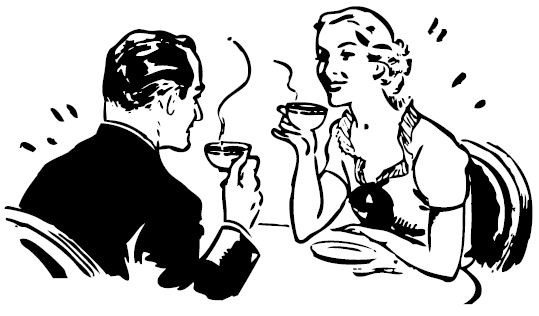
\includegraphics[width=\columnwidth]{kahvia.jpg}
\end{figure}
\subsubsection*{Cafe Tin Tin Tango}
\textit{Töölöntorinkatu 7}

Tinttarin ehdoton vetonaula on vuorokauden
ajasta riippumatta tarjolla oleva
aamiainen, johon kuuluu ääretön määrä
kahvia tai teetä. 2000-luvun alussa LiSuKe kokoontui täällä. Luettavana on Tinttisarjakuvia
ja taustalla soi klassista ja eteläamerikkalaista
tangoa. Takahuoneessa on
usein taidetta nähtävillä ja muita seiniä koristavat
Tintti-aiheiset taulut.
Tuolit ovat mukavia ja kännykkääkin
voi ladata jos akku loppuu. Myös pyykinpesu
onnistuu jos siltä tuntuu ja odotellessa
vaikka käväistä saunassa. Viihdykettä tarjoaa
baaritiskikin: A-oikeuksilla ja erityisesti
on mainittava laaja liköörivalikoima.
Asiakaskunta on kirjavaa ja sekalaisia julkkiksiakin
huhutaan nähdyn.
\subsubsection*{Café Ursula}
\textit{Ehrenströmintie 3}

Kaivopuiston eteläpäästä löytyvä kahvila
tarjoaa upean merimaiseman ja yleensä
kevään ensimmäisenä aukeavan terassin.
\subsubsection*{Espresso Edge}
\textit{Liisankatu 29}

Piristävän kirkkain värein sisutettu
kahvila, jossa ehdottoman kantispöydän
muodostaa kulunut sohvarykelmä. Täältä
saa todella hyvää minttukaakaota eikä kahveissakaan
ole valittamista.

\subsection*{Baarit ja pubit}
\subsection*{Kumpula}
\subsubsection*{Oljenkorsi}
\textit{Intiankatu 18}

Oljenkorsi on kampuksen lähin baari.
Sisustukseltaan ja tunnelmaltaan paikka
on perinteinen pubi varustettuna hyvällä
(pullo-)olutvalikoimalla. Paikka
on harvoin täynnä, joten sisälle mahtuu
isommallakin porukalla. Kesäterassilta voi
tuopin ääreltä katsella ohiajavia autoja ja
busseja ja päivitellä ihmisten kiirettä. Takahuoneessa
voi myös pelata biljardia. Tiistaisin
pubivisa.
\subsubsection*{Kipsari}
\textit{Hämeentie 135 E}

Aallon taiteiden ja suunnittelun korkeakoulun kellarikerroksessa
Arabianrannassa (kuutosen ratikan
päätepysäkin vieressä) sijaitseva pieni
baari/kuppila, jossa on päivisin tarjolla
opiskelijahintaista kasvisruokaa sekä iltaisin
kohtuuhintaista olutta ja varsin usein
livemusiikkia. Mainio paikka päästä osaksi
paikallisesta taiteilijailmapiiristä, ja harkinnan
arvoinen etenkin jos Unicafen (varsinkaan
kasvis)pöperöt eivät joskus satu
nappaamaan. Ruokalistat ja esiintyjät nähtävissä
osoitteessa: \url{www.kipsari.com}.
\subsubsection*{Ydinkeskusta ja Punavuori}
\subsubsection*{Thirsty Scholar}
\textit{Fabianinkatu 37}

HS kirjoitti huhtikuussa~2018: ``Opiskelijoiden juopottelu\-­toiminnasta ovat Helsingissä perinteisesti vastanneet osa\-kunnat ja aine\-järjestöt, joiden kerhotiloissa jäsenet ovat voineet toteuttaa kohtuu\-hintaista humaltumista valittuina ajan\-kohtina. [-{}-] Kaikista lähimpänä yli\-opiston omaa baaria on kuitenkin ollut Helsingin keskusta\-kampuksen Topeliassa sijaitseva kellari­krouvi\dots''

Ottamatta kantaa väitteen ensimmäiseen osaan, on kyseessä hyvin piilotettu ja siisti kivi\-jalka\-pubi yliopiston tiloissa, ja siksi se on erityisesti keskusta\-kampuksella opiskelevien suosiossa. Thirsty on sisustettu keski\-aika\-tyliin, ja asiakas\-paikkoja on reilusti. Sisäpihalla on suojainen terassi. Paikan omalla opiskelija\-kortilla saa euron alennuksen juomista, joten se haukkuu nopeasti hintansa takaisin.
\subsubsection*{Corona Baari}
\textit{Eerikinkatu 11}

Kaurismäen veljesten perustama ja elokuvateatteri
Andorran sisäänkäynnin luona
oleva baari. Täällä voit pelata biljardia lukuisilla
pöydillä, syödä toasteja ja odottaa
leffan alkua.
\subsubsection*{Kafe Moskova}
\textit{Eerikinkatu 11}

Aivan Coronan kyljessä sijaitsee tämä
pikkuruinen baari, myöskin Kaurismäkien
perustama. Tunnelma sen mukaisesti autenttisen
venäläinen kauhtuneine verhoiheen,
vanhoine vinyyleineen ja Lenin-tauluineen.
Tänne tullaan juomaan joko olutta
tai vodkaa, silloin kun kaikki on mennyttä
ja vain elämä itse jäljellä.
\subsubsection*{Molly Malone's}
\textit{Kaisanimenkatu 1C}

Hyvin suosittu irkkupubiketjun helsinkiläinen
jäsen. Joka ilta elävää bailausmusaa
ja ilmainen sisäänpääsy. Ei narikkaa arki-iltaisin
(viikonloppuisin pari euroa eteispalvelusta
joutuu pulittamaan). Asiakaskunta
erittäin kansainvälistä ja äänekästä.
Viikonloppuisin tänne on pitkä jono, kuten niin moneen keskustan paikkaan. Sisäpihalla suuri terassi, jossa kelpaa nautiskella lämpimästä kesäyöstä ja josta saattaa joskus saada ilmaista Guinnessiä.
\subsubsection*{Eerikin Kulma}
\textit{Eerikinkatu 28}

Harley Davidson meets John Wayne
meets Tuulipuku. Aito lähiökuppila keskustassa.
Halpaa olutta ja kapakkaruokaa.
Asiakkaina vakioita, teinejä ja vakioteinejä.
Sisustus koostuu hirsistä, pääkalloista,
neonvaloista ja yhdestä prätkästä (ei Harley).
\subsubsection*{Vanha}
\textit{Mannerheimintie 3B}

Vanhalla Ylioppilastalolla on kaksi
puolta: juhlatila ja Kuppila (nyk.\,Cafe
Vanha). Kuppilassa on yleensä ilmainen
sisäänpääsy. Oluita ja siidereitä löytyy ihan
kohtalainen valikoima. Juhlatilan puolella
on joskus bileitä ja keikkoja. Kesäisin on
Aleksanterinkadun puolella mukava kattoterassi.
\subsubsection*{Public House Black Door}
\textit{Iso Roobertinkatu 1}

Vuodesta 1992 alkaen toiminut olohuonemainen
Delifoxin laatupubi, joka on laajentunut
naapuriliiketilaankin. Black Door
valittiin Helsinki Beer Festivalin tuomariston
toimesta vuoden 2013 Olutravintolaksi.
Eikä syyttä, sillä valikoima kattaa n.\,200~pullo-olutta ja 24~hanaa, joista kahdessa on
real alea sekä kattava valikoima single malt
"-viskejä eikä laatusiidereitäkään ole unohdettu.
Täällä jos erehdyt tilaamaan sanoilla
``yksi tuoppi'', saat tyhjän tuopin.
\subsubsection*{Tommyknocker Craft Beer Bar}
\textit{Iso Roobertinkatu 13}

Helsingin olutraflojen trendin kärki
on vuonna~2015 Brewdogin baarin, Bier-
Bierin ja Tommyknocker Helsingin kolmio
muillekin kuin IPAa kyseleville oluthipstereille.
Tommyknockerin erikoisuus on,
että se on panimonsa ensimmäinen ravintola
Coloradon Idaho Springsin ulkopuolella.
Kalaravintoloilla (niistä ei kalaa saa)
kuuluisaksi tulleella Delifoxilla on tosin
lusikkansa maltaissa, sillä Tommyknocker
kuuluu Delifoxin ketjuun kuten läheinen
Black Door. Ainutlaatuiset oluet ja mielenkiintoiset
suomalaiset pienpanimotuotteet
ja tiskin sijasta takaseinälle asennetut hanat
yms.\,trendikästä. Kannattaa käydä katsomassa
ja kapakasta voi ostaa mukaan root
beeria.
\subsubsection*{Karaokebar Erottaja}
\textit{Erottajankatu 15--17}

Erottajalla tuntuu olevan aina porukkaa.
Sisustus on melko trendikäs tiiliseinineen
ja metallisine pikkupöytineen, mutta
kuitenkin tunnelmallinen valaistuksen ja
tiiviin kalustuksen vuoksi. Olut on kohtuuhintaista
ja lisäksi löytyy pikkupurtavaa,
kuten äärimmäisen herkullisia toasteja.
Oman soittolistan musiikki oli melko lujalla,
mutta ei häirinnyt keskustelua.

\subsubsection*{Virgin Oil}
\textit{Mannerheimintie 5}

Ulkoasultaan varsin tyylikäs baariravintola,
jossa myös Limeksen vappubileitä
on pidetty ja Limeksen approssa kierrelty.
Paikan kävijäkunta ei tee oikeutta sen hienoille
mutta koville tuoleille. Ravintolassa
on myös paljon pehmoisia sohvia, mutta ne
ovat kaikki yleensä vallattuina. Täältä saa
usein halpaa skumppaa ja viiniäkin. Lisäksi
melko nimekkäätkin bändit tapaavat esiintyä
Virgin Oilissa. Kuten mainoslause toteaa:
``From dining to stage diving''
\subsubsection*{Zetor}
\textit{Mannerheimintie 3--5 (Kaivopihan UniCafen vieressä)}

Jos olet kotoisin sieltä missä lehmänpaska
haisee ja valmetti valittaa, kannattaa
koti-ikävän iskiessä pistäytyä Zetorissa.
Paikka on hyvin maalaishenkinen jo pelkästään
lähtien sisustukseen kuuluvista
vanhoista Zetor-traktoreista. Ruokalistalta
löytyy hyvin suomalaista perinteistä ruokaa
ja juomaksikin ainakin toisinaan on saatavilla
sahtia. Viikonloppuisin paikka täyttyy
juhlivista keski-ikäisistä. Erittäin tyylikäs
miesten wc.
\subsubsection*{Aussie Bar}
\textit{Salomonkatu 5}

Täällä voit tavata aidon aussin, sillä
ainakin yksi baarimaija on sellainen. Saat
myös kuulla ja puhua englantia ja maksaa
juomista melko paljon.
\subsubsection*{Mann's Street}
\textit{Mannerheimintie 12 A}

Vanhempien (homo)miesten kohtauspaikka
Helsingin keskustassa. Ei silti haittaa,
vaikka olisit nainen. Karaoke on melko
tasokas ja laaja valikoimaltaan.
\subsubsection*{Navy Jerry's}
\textit{Hietaniemenkatu 2}

50-luvun henkeen sisustettu merimiesravintola.
Suositeltava kohde rommin ystäville laajan valikoiman ansiosta. Rommishower on erityisen hyvä drinkki (sisältää raakaa kananmunaa), jolla saa helposti poltettua viikon ruokabudjetin verran yhdessä illassa.
Fiftareiden suosiossa, mutta musiikki on
useammalta vuosikymmeneltä. Keskustan
hintatasosta huolimatta ajoissa pitää tulla,
jos haluaa mahtua istumaan. Huom! Ikäraja
22~v., mihin ei järjestön (HAO~ry) exculla
saatu etukäteen neuvottelemalla helpotusta.

\subsubsection*{Pub Pete}
\textit{Hietaniemenkatu~7}

Ennen Pub Pete oli kauhea läävä, nykyään se on pastelli\-väreillä päällystetty limeenvihreä hipsteribaari, jossa saa laulaa karaokea joka päivä. Matlu-klusterin lähibaari, jota kannattaa yrittää, jos ikä ei riitä Navy Jerry'siin.

\subsubsection*{Stone's Gastropub}
\textit{Keskuskatu~4}

Hanaoluita ja rasvaista herkkuruokaa.
``Herkkuruoasta'' Hesarin toimittaja totesi
Nyt-liitteessä: ``Olen nyt kolme kertaa
käynyt täällä syömässä, enkä neljättä kertaa
tule''. Suosituimmat oluet näkyvät reaaliaikaisella
olutmittarilla, jonka mukaan
hanatuotteita tilataankin. Mikäli sinulla on älypuhelin, niin muista myös Foursquare-tarjoukset!
\subsubsection*{Töölö}
\subsubsection*{Bar Fellows}
\textit{Mannerheimintie~64}

Kisahallia vastapäätä olevan Bar Fellowsin
sisustukseen on panostettu sen
verran, että tavallisten baarituolien sijaan
paikka on varustettu mukavilla nojatuoleilla.
Urheiluhenkisille baariin on asennettu screeni ja pari televisiota. Varsinkin ennen
suurempia jalkapallotapahtumia Fellows on usein varsin täynnä.
\subsubsection*{Ølhus Helsinki}
\textit{Mannerheimintie~104}

Skandidaavinen baari Taka-Töölössä.
Vanhan jäähallin läheinen sijainti houkuttelee
paikalle HIFKin tsekkivahvistuksia.
Hyvä olutvalikoima, viihtyisä sisustus ja
syrjäinen sijainti takaavat mukavan tunnelman.
\subsubsection*{KuuKuu}
\textit{Museokatu~17}

Museokadulla sijaitsevalla KuuKuulla
on sellainen maine, että siellä hengailee paljon
taiteilijoita, sekä wannabee-taiteilijoita,
jotka kertovat tarinoita kuinka he ovat istuneet
iltaa kuuluisien taiteilijoiden kanssa.
Paikalla on myös taidenäyttelyitä. Jos sattuu
olemaan Töölössä päin pyörimässä
niin ehdottomasti kokeilemisen arvoinen paikka. Kannattaa myös kokeilla paikan keittiö.
\subsubsection*{St Urho's Pub}
\textit{Museokatu 10}

St Urho's Pub kuuluu Bottan ravintola-
ja baarirykelmään. Urho on erityisesti
olutravintola,
mikä ilmenee laajasta hanavalikoimasta,
johon kuuluu kaksi real ale
"-hanaa. Lisäksi valikoimassa on laaja pullo-olutvalikoima
ja sahtia. Urkki on vuoden~2006 Olutravintola (Helsinki Beer Festivalin
tuomaristo). Tunnelma ja sisustus on
hyvin peruspubimainen. Taustamusiikkia
Urkissa ei ole, mistä hyvästä Helsingin
Muusikot~ry on myöntänyt Hiljaisuus "-palkinnon
Urkille, ja asia on eriyismainintana
Vuoden Olutravintola palkinnon perusteluissa.
Ruokalistalta löytyy kaksi kertaa
pizzalautasta suurempia pizzoja, isoja salaattiannoksia.
Lieneekö Urkki Suomen ainoa kunnon pubiruokaa tarjoileva laatuolutpubi.
Kuten sijainnista voi päätellä,
hintataso on varsin korkea. Henkilökunta
on asiantuntevaa, muttei väheksy olutkulttuurista
vähemmän tuntevaa asiakasta (viinilasi
huuhdeltiin tuopin huuhtelulaitteella \smiley). Asiakaskunta on sivistynyttä, Arto Nybergin
kantapaikka.
\subsubsection*{Vastarannan Kiiski}
\textit{Runeberginkatu~26A}

Vastarannan kiiski on letkeän
tunnelmallinen
pubi, joskin hieman kalliin
puoleinen. Hyvä juoma- ja pelivalikoima
lämmittävät sydäntä, jos illalta halutaan
muutakin kuin halvat räkäläkännit. Suhteellisen
kattavan hana- ja pullovalikoiman
lisäksi ravintolasta löytyy lämpimiä toasteja,
joilla on mukava hillitä suolahimo. Ikäraja
on viikonloppuisin
20~v.

\subsubsection*{William K.}
\textit{mm.\,Mannerheimintie~72}

Tämä viihtyisä olutravintola on sisustukseltaan
jotenkin olohuonemainen mutta
sillä erolla, että matot on sijoitettu pöydille.
Tiskin takaa löytyy vaikuttava valikoima
oluita ja viskejä -- laatuakin on tarjolla,
jos kukkaro kestää varsin suolaiset hinnat. Tämä on myös Helsingin harvoja paikkoja, josta saa tuoretta sahtia.
Myös paikan kuuluiset jättitoastit ovat tutustumisen
arvoisia. Tilavannäköisestä
ravintolasta löytyy luultavasti aina vapaa
pöytä, ehkä lukuunottamatta iltoja, jolloin
se on stadikalta virranneiden jalkapallofanien
täyttämä. Samannimisiä ja muutenkin
toisiaan muistuttavia paikkoja löytyy
Helsingistä neljä kappaletta mutta tämä on
niistä vanhin ja parhailla valikoimilla varustettu.
\subsection*{Ruoholahti}
\subsubsection*{One Pint Pub}
\textit{Santakatu~2, Sinikaislankujan puoli kanavan
vieressä}

Räkälä, jolla on oma olutmaahantuonti
ja valikoimassa maailman ainoa tyrnimarjalambic,
jota Cantillon panee vain Pinttarille.
Omistaja Markku Korhonen on Helsingin
Beer Festivalin pääjärjestäjä, ja on
aloittanut oluturaansa Vanhan Kuppilassa
80-luvulla, kun Vanha oli johtava laatuolutravintola.
Näin oli vuoteen~2014 asti. Nyt
Korhosella on vain pieni vähemmistöosuus,
ja ent.\,työntekijät omistavat kapakan.
Viestintä nettisivujen (\url{www.onepintpub.com/olutvalikoima}) ja naamakirjasivun kera
on parantunut, mutta oma maahantuonti
on supistunut, sillä enää ei Korhonen lähde
kuorma-autolla kierrokselle Euroopan
panimoihin keräämään teemaolutviikoille
ainutlaatuisia oluita. Pinttarissa silti ainutlaatuisina
oluina on edelleen De Proef
brouwerijin Redneck (talon olut) ja
Malmgårdin Alpo's IPA (Kirjailija Alpo
Ruuthin muistolle).
Muutoksista huolimatta Pinttarissa edelleen
keskitytään laatuoluisiin. Trendisisustusta
ja snobbailua harrastavat älköön vaivautuko.
Kesäisin on käytössä iso terassi
kanavan lähellä.
\subsection*{Oulunkylä}
\subsubsection*{Olutravintola Jano}
\textit{Mäkitorpantie~11}

Oulunkylän ja Käpylän rajalla (Käpylän
asemalta lyhyempi kävelymatka) sijaitseva
kohtuullisen uusi yksityinen laatuolutravintola.
Rähjäinen ja kulunut sisustus,
mutta kova on omistajalla yritys kehittää
raflastaan olutpiireissä suosiota saavaksi.
Nähtäväksi jää, että kaatuuko sijaintiinsa.
Palvelu (omistaja tiskin takana) oli ystävällistä,
asiantuntevaa ja humoristista. Hintataso
on keskustan laatuolutravintoloita hieman
edullisempi.
\subsection*{Kallio}
Kun Helsingissä tekee mieli mennä kaljalle
muttei maksaa itseään kipeäksi, kannattaa
suunnata Kallioon. Kun haluaa ehdottoman
rentoa (joskus jopa liian rentoa)
menoa kaljan ja pizzan merkeissä, kannattaa suunnata Kallioon. Siellä kadut vilisevät
kaljakuppiloita, pizzerioita ja kebabboloita.
Hinta-laatusuhde on Kalliossa melko
kuvaava. Jos haluat halvimman mahdollisen
tuopin, saat myös kestää örinät ja melko
harmittomat baaritappelut, sekä tietenkin
haisevat vessat. Mitä enemmän suostut
tuopistasi maksamaan, sitä rauhallisempaa
ja sivistyneempää ympärilläsi on. Jos siis
jostain syystä pidät rauhasta ja sivistyksestä.
\subsubsection*{Iltakoulu}
\textit{Vaasankatu 5}

Iltakoulu on kalliolaisista paikoista siitä
siistimmästä päästä, tuopin hinnan pysyessä
kuitenkin vielä kohtuullisena. Kallionkävijät
rankkaavat paikan rokkaavan
jukeboksin alueen parhaimpiin, ja henkilökunnastakin
on puhuttu pelkkää hyvää. Kaiken lisäksi paikan wc on kenties kaupunginosan
siistein. Tyyliltään Iltakoulu
on presidenttien metsästysmaja: kattokruunuja,
tummaa puuta, loosseja, sekä täytettyjä
eläimiä ja presidenttien muotokuvia. Terassi
on varsin viihtyisä, tosin aurinkoisena
päivänä aina täynnä: sinne nimittäin paistaa
aurinko varsin pitkään. Kuten monesta
muustakin paikasta, täältä löytyy baariillan
virkistykseksi
lautapelejä, mm.\,Trivial Pursuit. Ei erityisempää happy houria.
\begin{figure}[h!]
	\centering
	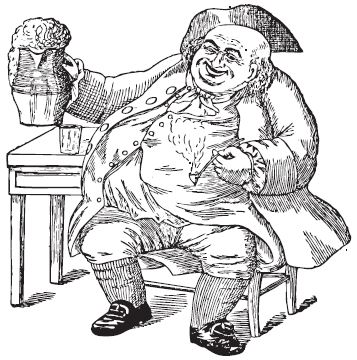
\includegraphics[width=\columnwidth]{tuoppimies.jpg}
\end{figure}
\subsubsection*{Mascot Bar}
\textit{Neljäs linja 2}

Mascot sulkeutui yllättäen heinäkuussa 2017, mutta avautui uudelleen joulukuussa omistajanvaihdoksen jälkeen. Entinen Cafe Mascot on oiva valinta niille, jotka tykkäävät viettää baarissa aikaa pelejä pelaten tai livemusiikkia kuunnellen. Pelinnälkäisille valikoimassa on parikymmentä erilaista lautapeliä, biljardipöytiä ja jopa autopelejä. Lisäksi baarissa järjestetään maanantai-iltaisin kielikahvila jossa väkeä onkin paikalla runsaasti. Paikka on suurempi kuin miltä ulospäin näyttää, ja MaO ja muut ainejärjestöt varaavat usein sen yläkerrasta pöytäryhmän yksityistilaisuuksiin.
\subsubsection*{Om'pu}
\textit{Siltasaarenkatu~15}

Om'pu tarjoaa asiakkaalleen keskusteluun
sopivan hiljaisen musiikin puolen. Screeniltä
voi joskus nähdä esimerkiksi South
Parkia. Naapureitaan
siistimpi ja trendikkäämpi
sisustus tosin nostaa hinnat korkeammiksi
kuin Kalliossa yleensä.
\subsubsection*{Pub Sirdie}
\textit{Kolmas linja~21}

Miniatyyriravintola kolmannella linjalla,
tilaa noin viidelletoista. Populaarimusiikista
huolehtii jukeboksi, eurolla saa valita kaksi seiskatuumaista hienosta valikoimista.
Hyvin intiimi paikka.
\subsubsection*{Stellar}
\textit{Helsinginkatu~21}

Stellar ei ole kokenut remonttia aikoihin,
ja vessa oli kamala. Rähjäisen näköinen
paikka yllättikin loistavalla palvelulla:
lonkunkin saa vaikka kahteen lasiin kaadettuna
ja terassille lisäpöydän tilan loppuessa!
Sisäpuolen sisustus on outo: suurin osa
vähistä tuoleista on sijoitettu seinän vierustalle
lukuunottamatta paria pientä pöytää,
joten tunnelma on jotain AA-kokouksen
ja Amsterdamin coffee shopin väliltä. Asiakaskunta
on pääasiassa rentoa nuorisoa.
Hinnat ovat alueen keskitasoa, ja paikalta
löytyy myös biljardipöytä mikäli pelkkä
oluen juominen kyllästyttää.
\subsubsection*{Bar Bronco}
\textit{Hämeentie 23}

Tämä melkein Kurvista löytyvä urheilupaikka
on aika lailla keskinkertainen paikka lukuun
ottamatta lokoisaa takahuonetta, jossa
on varsin mukava kattella futista. Jukeboksi löytyy ja muutama
peli. Paikan varsin ahtaasti sijoitetut
pöydät on pultattu lattiaan kiinni.
\subsubsection*{Pub Porthan}
\textit{Porthaninkatu 10}

Portsu on oikea kunnon räkälä. Ei niin,
että siinä olisi mitään erityisen pahaa. Sisustus
on mauton, vessa saastainen ja olut
halpaa. TV:stä näytettiin Salkkareiden
uusintoja, mikä ei miellyttänyt allekirjoittanutta
alkuunkaan. Kyllä täällä kuitenkin
voi mainiosti kaljaa kitata, silloin kun siihen
on tarve.
\subsubsection*{Kallion Oiva}
\textit{Porthaninkatu 5}

Riippuen siitä onko karaoken ystäviä vai
ei, tänne joko kannattaa hakeutua tai tätä
paikkaa kannattaa karttaa arkisin klo 22--24, pe klo 19--24,
la klo 18--24 ja su klo 15--24. Itselleni tuli
melkoinen kiire saada tuoppi tyhjäksi, kun
kello löi seitsemän ja kaiuttimista pärähti
niin sielukas tulkinta jostain tunnistamatta
jääneestä biisistä että oksat pois. Oivassa
on euron narikkamaksu ja Kallion mittapuulla
hintavaa olutta mutta toisaalta myös
paljon tilaa, nahkasohvia ja darts-taulu.
Tänne voi siis tulla vähän isommallakin
seurueella iltaa istumaan. Discopallosta tulee
lisäpisteitä.
\subsubsection*{Olutravintola Sivukirjasto}
\textit{Fleminginkatu 5}

Sijaitsee Kallion kirjaston takana ja ilmoittaa
tarjoavansa 100~vaihtoehtoa kirjoille.
Sivukirjasto on siististi sisustettu
laatuolutravintola, jonka mukainen toki on
hintatasokin. Pubivisan aikaan on kuin ammuttu
täyteen, ja paikalta voi bongata myös kuuluisia vasemmistopoliitikkoja.
\subsubsection*{Ravintola Toveri}
\textit{Castreninkatu 3}

Kolmannen linjan varrelta löytyvä Toveri
hakee sisustuksessaan 70-lukulaista vasemmistotyyliä osin siinä myös onnistuen.
Seurueemme huomion kiinnittää kuitenkin
asiakaskunnan ilmiselvä porvarillisuus.
Tämähän on kuitenkin hyvin
linjassa demarien nykyisen politiikan kanssa,
joten mitä siitä valittamaan. Hanasta on
saatavilla hyvä valikoima ulkomaisia oluita
varsin kohtuulliseen hintaan. Toveri tarjoaa
myös pikkunaposteltavaa, tapaksia ja monenlaisia
drinkkejä, jos joku niitä Kalliossa
keksii kaivata. Maksuvälineeksi ei käy Visa
Electron, mikä tarkoittaa useilla opiskelijoilla
kävelyretkeä lähimmälle pankkiautomaatille.
Kokonaisuutena Toveri on varsin
miellyttävä paikka keskustella ja nauttia
hyvää olutta.
\subsubsection*{Roskapankki}
\textit{Helsinginkatu 20}

Roskapankki eli Roskis on melko tunnettu
baari Brahenkentän läheisyydessä.
Asiakaskunta
on suurimmalti osin keski-ikäistä.
Olut on erittäin halpaa ja paikka aukeaa
jo yhdeksältä. Musiikki soi melko kovalla
jo aika alkuillasta. Mielenkiintoiseksi
vierailun tekee naisten vessan peilit, jotka
sijaitsevat koppien takaseinillä. Juomien
hinnat ovat Kallion halvimpia. Kesäisin iso
terassi joka on usein täysi. Täältä saa myös
pitsaa jos ei pelkää salmonellaa.
\subsubsection*{Panema}
\textit{Helsinginkatu 11}

Mennäänkö Panemaan? Tämä tammikuussa 2018 avattu craft beer "-paikka sijaitsee kävelymatkan päässä Sörkän
metroasemasta. Vaaleat puupöydät tuovat paikkaan kliinistä tunnelmaa. Siisti vessa,
vaihtelevaa musiikkia. Henkilökunta on englanninkielistä ja hyvin palvelualtista -- suomalaiset eivät epäilemättä jaksaisi kuunnella baarin nimeen liittyviä vitsejä päivästä toiseen\dots
\subsubsection*{Kallion Pörssi}
\textit{Alppikatu 17}

Hieman rauhallisemman näköisellä
paikalla sijaitseva Pörssi on sisustukseltaan
kierroksen makein: punaiset sohvat,
ihanat punamarmoriset pöydät, katossa
jotain mielenkiintoista sekä Suomen lippu
seinällä. Musiikkia jukeboksista. Miinusta
naisten vessan hankalasta ovesta ja märästä
lattiasta, miesten wc kierroksen heikoin:
kansi sidottu jessellä. Narikka ke--la 1~\euro.
Häppäri 10--19. Hinnat normaalia Kallion
tasoa.
\subsubsection*{Helsing Bar}
\textit{Kaarlenkatu 3--5}

Rennonletkeä baari mukavalla henkilökunnalla. Seiniä koristaa vinyylilevyt, ja taustalla soi vaihtoehtorock, folk rock ja garage rock. Erittäin vajaa kolmostuoppi \EUR{3,50}. Tilassa toimi aiemmin Helsingin ainoa lesbobaari Nalle-Pub, ja sen jäljet näkyvät asiakaskunnassa edelleen.
\subsubsection*{Majava-baari}
\textit{Porthaninkatu 9}

Rokkarien suosima roudaribaari. Paikanpäältä voi usein bongata suomalaisia rockja
metallivaikuttajia.Kalja sopihintaista ja
rokki soi. Legendaarinen jukeboxi käyttöohjeineen.
\subsubsection*{Siltanen}
\textit{Hämeentie 13 B}

Rento baari ja klubi, jossa kuulee usein livebändejä ja hyviä DJ:tä. Päivisin Siltasesta saa kohtuuhintaista lounasta, ja terassi on aurinkoinen.
\subsubsection*{Kuudes Linja}
\textit{Hämeentie 13}

Kutonen on Siltasta isompi ja yökerhomaisempi. Koska Siltasen ja Kuudennen linjan välissä kulkee rappuset, on helppo tsekata molempien baarien tarjonta saman illan aikana. Esiintyjät keräävät viikonloppuisin kadulle satojen metrien mittaisen jonon ja sisällä joutuu olemaan tappituntumalla.
\subsection*{Musiikkia}
\subsubsection*{Tavastia}
\textit{Urho Kekkosen katu 4--6}

Aiemmin Hämäläis-Osakunnan omistuksessa ollut, maan suurin ja mahtavin rock-klubi,
jonne kaikki suomalaiset bändit tahtovat
esiintymään. Vähemmän nimekkäät bändit
esiintyvät takapihan Semifinalissa.
\subsubsection*{Nosturi}
\textit{Telakkakatu 8}

Elävän musiikin yhdistyksen ELMUn
ylläpitämä keikkapaikka, missä esiintyy
usein myös ulkomaisia bändejä.
\subsubsection*{On the Rocks}
\textit{Mikonkatu 15}

Rokkia ja stand-uppia. Mukavan intiimi
klubi, jossa ohjelmaa keskiviikosta lauantaihin.
Hintataso ei mikään edullinen, mutta
Happy Hour "-kantakortilla joskus hyviä
tarjouksia.
\subsubsection*{Lepakkomies}
\textit{Helsinginkatu 1}

Rokkia ja halpaa kaljaa Hesarilla.

\begin{figure*}[!b]
	\centering
	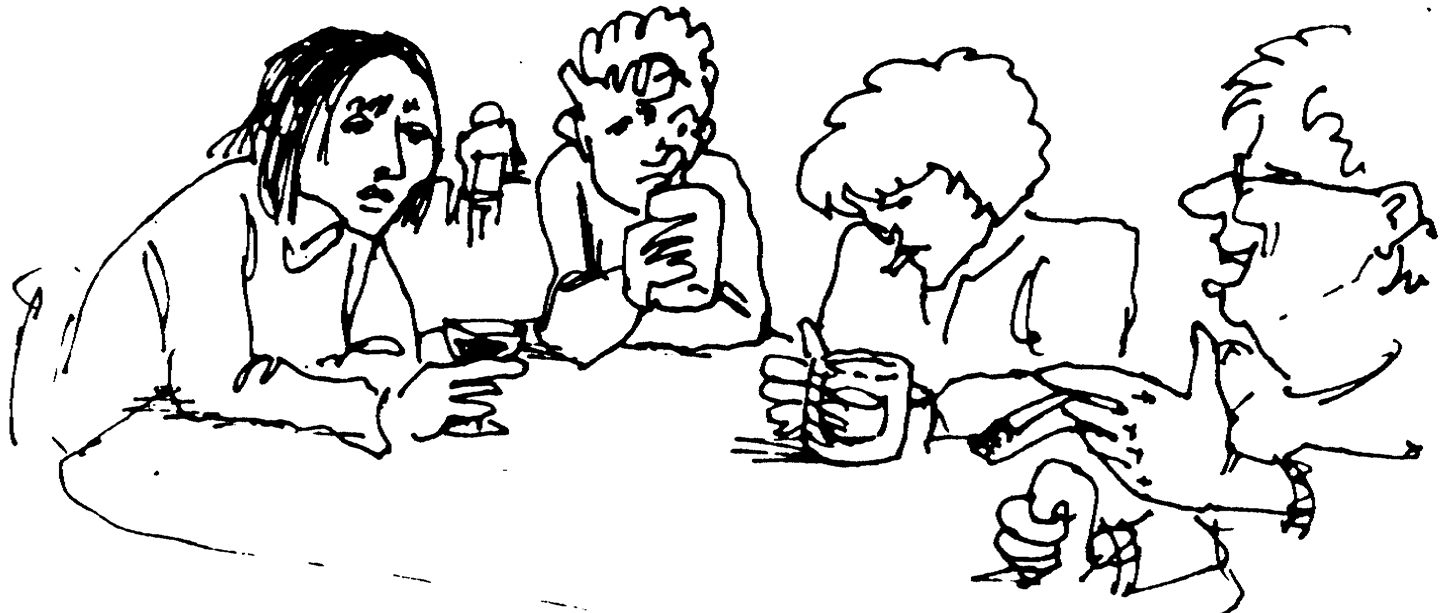
\includegraphics[width=\textwidth]{juovatringissa.png}
\end{figure*}
\subsection*{Metrokierros}
Porukka limettejä päätti eräs kesäinen
päivä lähteä tarkistamaan millaisia baareja
metroasemien läheltä löytyy. Päätimme
lähteä liikkeelle Itäkeskuksesta kohti keskustaa, sillä arvelimme että emme kuitenkaan
kerkeäisi Ruoholahteen asti edes
Itäkeskuksesta ennen kuin metro lopettaa
liikkumisensa. Ja oikeassa olimme, emme
päässeet edes Rautatientorille, mutta alla
arvioita paikoista joissa vierailimme. Kaikki
paikat sijaitsevat siis mahdollisimman
lähellä metroasemia.
\subsubsection*{Ravintola Siilinpesä}
\textit{Siilitie M}

Siilitien metroasemalta alas tullessa kun
kääntyy oikealle, niin sadan metrin päässä
tien toisella puolella näkeekin jo ravintola
Siilinpesän. Paikka vaikuttaa ulospäin melko
kodikkaalta lähiöravintolalta, jossa on
terassi. Erikoisuutena kuitenkin tässä paikassa
on erinomainen ruoka, varsinkin lounaspöytä
on herkullinen. Jos koskaan satut
olemaan lähistöllä liikkeellä niin kannattaa
käydä kokeilemassa!
\subsubsection*{Treffipub}
\textit{Herttoniemi M}

Treffipub näkyy suoraan Herttoniemen
metroasemalta, yksi tie täytyy ylittää että
pääsee paikalle. Paikka on melko lailla peruslähiöbaari,
jossa ikäraja on 20~v.\,ja musiikin
taso vaihtelee laidasta laitaan. Paikasta
löytyy myös yksi biljardipöytä. Paikassa
käy todella heterogeenistä jengiä. 

Yksi
erikoinen huomio paikasta tehtiin: Naisten
vessa on miesten suunnittelema, peili pään
takana, ei näe mitään kun meikkaa. Hana
valuu aina ja käsienkuivauskone
hyökkää.
Mutta ihan siisti.
\subsubsection*{Kuparilyhty}
\textit{Kulosaari M}

Kulosaaren metroaseman ja Kuparilyhdyn
välissä on useita satoja metrejä villiä
luontoa, sillä paikka sijaitsee Kulosaaren
ostoskeskuksessa.
Kuparilyhdystä saa ihan
hyvää pizzaa, mutta drinkkivalikoima on
erittäin suppea, muun muassa mansikkamargaritaa
ei paikassa saanut. Asiakaskunta
on hieman vanhemmanpuoleista, opiskelijaördääjiä
paikassa ei ollut.
\subsubsection*{Kurvitar}
\textit{Sörnäinen M}

Kallion nurkille tullessa baarien tiheys
nousee yhtäkkiä todella suureksi. Metroasemalta
suuntaamme Kurvittareen, joka
on muutaman askeleen päässä Sörnäisten
metroasemalta. Lähempääkin olisi löytynyt
baareja. Kurvitar on Kallion perusräkälöitä,
papereita tiedusteltiin tosin aika ahkerasti.
Paikasta ei keskimäärin pidetty kauheasti,
olut maistui pahalta ja naisten vessassa oli
huumevalot. Olut tosin oli halvinta koko
kierroksella, mutta tämähän on Kalliota.
\subsubsection*{Kaisla}
\textit{Helsingin yliopiston M}

Kaisaniemen asemalta noustessamme
päätämme suunnata olutravintola Kaislaan.
Kaislassa on tosiaan paljon erilaisia oluita
tarjolla, mutta hintataso tuntuu Kallion
jälkeen melkoisen kovalta. Taustalla soiva
musiikki on mukavaa, eikä liian kovalla,
keskustelu onnistuu hyvin. Sisustus on tyylikäs
ja paikka on erittäin siisti. Jos siis varasi
riittävät ja haluat istua mukavasti iltaa,
niin Kaisla on hyvä paikka Rautatieaseman
vieressä, eli hyvien liikenneyhteyksien varrella. Kaisla on HOK-Elannon Oluthuoneista
paras, vaikkakin hanavalikoima on
pysynyt melko samana n.\,10 vuotta. Kaisla
on Akateemisen Olutseuran (AOS) kantaravintola
vuosilta~2007--2009 ja jälleen
vuodesta~2012 alkaen. AOSlaisia löytää
Kaislasta joka kuukauden ensimmäisenä
sunnuntaina kuukausitapaamisessaan.

\subsection*{Metrokierros, vol.\,2}
Länsimetron ensimmäinen vaihe avattiin marraskuussa~2017, ja useampikin Limes-aktiivi oli mukana metron ensimatkalla -- jota teekkarien takia myös neitsyt\-matkaksi kutsutaan. Vuoden 2018 kesäkuussa Ähiksen toimitus päätti lähteä jatkamaan aiemmin kesken jäänyttä ravinteli\-tutkimusta Kampista länteen. Erotukseksi edelliskerrasta kierroksella päätettiin ensisijaisesti tunnustella baarien atmosfääriä sekä taustamusiikkeja ja keskittyä muuten lähinnä tavan\-omaisimpiin hana\-tuotteisiin.

Yleisesti voidaan todeta, että baarissa kannattaa aina tehdä muistiin\-panoja, koska sitten sinua luullaan Helsingin Sanomien toimittajaksi, ja saat parempaa palvelua.
\subsubsection*{Oluthuone Amsterdam}
\textit{Ruoholahti M}

Purjehdus\-henkinen paikka aivan Ruoho\-lahden metro\-aseman kyljessä. Hana\-valikoima vaikuttaa monipuoliselta, ja asiakas\-paikkoja on reilusti, myös terassilla. Asiakas\-palvelu oli myös toimivaa. Sisällä huomio kiinnittyy nopeasti katossa olevaan Litmasen peli\-paitaan -- Litihän on iso nimi Alanko\-maissa Ajax-uransa takia. 

Soittolista:
\begin{itemize}
	\item Shura: Touch (2016, electropop)
	\item Michael McDonald: Hail Mary (2017, blue-eyed soul)
	\item Ciara: Gimmie Dat (2010, electrodance)
	\item Limp Bizkit: Behind Blue Eyes (2003, rock)
\end{itemize}
\subsubsection*{Pub Pikku Katti}
\textit{Lauttasaari M}

Pikku Katti on kiva pikku lähiö\-pubi, josta löytyy myös TV, juke\-boksi ja tieto\-kone. Paikka on oikeasti pieni, mutta terassilla on myös istuma\-paikkoja jos tila loppuu sisältä. Urheilua kannattaa ehkä mennä katsomaan jonnekin muualle kuin tänne, mutta tuopillisen Karhua saa kyllä melko halvalla.

Koska Koivu\-saaressa ja Keila\-niemessä ei oikein ole baareja, hypättiin kahden seuraavan aseman yli ja jäätiin vasta Ota\-niemen pysäkillä. Otaniemessä tutustuttiin myös metro\-aseman WC-tiloihin, joita varten pitää olla tekniikan kandin paperit, että niitä osaa käyttää. Kansi nousee ja laskee napin painalluksella, ja käsien\-pesu\-vesi ja paine\-ilma suihkuavat seinässä olevasta aukosta.

\subsubsection*{Fat Lizard}
\textit{Aalto-yliopisto M}

Uusi iso panimo\-ravintola aivan metro\-asemaa vasta\-päätä. Fat Lizardin omat pale alet ovat Espoon ylpeys, ja valikoima vaihtuu tiheään. Keittiö on valtava ja jokaisena vuoden päivänä auki ainakin keskiyöhön. Viikon\-loppuisin kuuluisia pizzoja saa kuulemma aamu\-neljään asti. Vasta\-painona on kalliit hinnat ja heikko asiakas\-palvelu. Baari\-nurkkaus on melko ahdas.

Soittolista:
\begin{itemize}
	\item Umii: Dangerous (2017, R\&B)
	\item The Endorphins: Ms.\,Right Now (2017, R\&B)
	\item Majid Jordan: Make it work (2016, synthpop)
	\item Sam Wills: Electrified (2016, R\&B, house)
	\item SG Lewis ft.\,Gallant: Holding Back (2016, electric dance)
\end{itemize}
\subsubsection*{Sherlock}
\textit{Tapiola M}

Tapiolan metro\-asemalla ihminen kokee kyllä itsensä pieneksi. Sherlock on aivan kiven\-heiton päässä asemalta, mutta se on hyvin piilossa kerros\-talon pohja\-kerroksessa. Ulkoa päin paikkaa ei välttämättä tunnistaisi baariksi. Henkilö\-kunta on hauskaa, ja Sherlock vaikuttaakin hyvältä after\-work-paikalta. Tausta\-musiikki miellytti alle\-kirjoittanutta, jonka musiikki\-maku on jämähtänyt pysyvästi 1970-luvulle. Ainoana miinuksena todettakoon, että asiakas\-puolella ei ole pisto\-rasioita.

Soittolista:
\begin{itemize}
	\item Clarke/Duke: Wild Dog (1981, jazz)
	\item Duke: I love you more (1979, pop-funk)
	\item Tina Charles: I love to love (1976, disco, bossa-nova)
	\item Labelle: Lady Marmalade (1974, soul)
	\item Melba Moore: This is it (1976, disco)
\end{itemize}

Niittykummun ja Urheilu\-puiston asemien läheltä ei vaikuttanut löytyvän anniskelu\-ravintoloita, joten nämäkin hypättiin suoraan yli, ja matka jatkui päättärille asti.

\subsubsection*{Krouvi Fortuna}
\textit{Matinkylä M}

300~m kävelymatkan päästä Länsi\-metron pääte\-asemalta löytyy melkoisen tilava pubi, jossa on reissun halvin tuoppi, ja jossa vaikuttaa video\-tykin ja mikseri\-nurkkauksen perusteella olevan viikon\-loppuisin myös karaoke\-mahdollisuus. Google Maps valehtelee paikan olemassa\-olosta.

Soitto\-listalla oli reissun ainoana myös pohjois\-maista musiikkia:
\begin{itemize}
	\item Laura Voutilainen: Mä en kestä (2017, pop)
	\item Avicii: Levels (2011, progressive house)
	\item Usher: More (2011, Hi-NRG)
	\item Profeetat ft.\,Nelli Matula: EYO (2017, hip hop)
	\item Katy Perry ft.\,Nicky Minaj: Swish Swish (EDM)
\end{itemize}
\subsection*{Itä-Helsinki}
\subsubsection*{New Stone}
\textit{Humikkalanrinne 1}

Nightclub Stone on vapaa-aika\-virasto.comin mukaan Suomen toiseksi paras ja
Helsingin paras yökerho. Silti on erikoista,
ettei miltei kukaan ole käynyt siellä! Tämä
voi johtua siitä, että se sijaitsee Itä-Helsingissä
kohtalaisen kävelymatkan päässä
etäisimmästä metroasemasta. Tästä huolimatta
hyvin mukava, pieni yökerho, jonka
palvelu on mukavaa. Bonuksena paikan
vessa on hyvin siisti läpi yön! 

``One of the hot spots of the Helsinki club/disco scene.
It has everything you might imagine, including
noise and imperfect air-conditioning.''
\footnote{\url{www.professionaltravelguide.com}}
\subsubsection*{Aapelin baari}
\textit{Ostostie 4}

Aapelin baari on Kontulan ostoskeskusta
määrittävä baari, jossa jokainen katu-uskottava
kontulalainen on käynyt. Tämä voi
siis olla hyvinkin huono asia. Paikan erikoisuus
on ystävällinen henkilökunta, joka
tarjoilee juotavaa vaikka kolmen promillen
humalassa oleville asiakkaille!
\subsubsection*{Pikkulintu}
\textit{Klaavuntie 11}

Puotilan ostoskeskus on kummallinen
paikka -- siellä on palkittu kebab-paikka,
vietnamilaisen perheen ruokaravintola
Com Viet ja nukketeatteri Sampo, jossa
Japanin keisarinna on käynyt seuraamassa
nukketeatteriesitystä -- ja siellä on Olutravintola
Pikkulintu. Olutravintola isolla
O:lla, sillä Pikkulinnun olut- ja mallasviskivalikoima
on maahantuonnin ansiosta
varmasti Suomen parhaimmistoa! Hanavalikoima
vaihtuu kuukausittain tai tiheämmin,
mutta Plevnan Siperia pysyy ja opettaa.
Pikkulintu on paikka, jossa on käytävä
ennen valmistumista. Meridiaanin puolivirallinen olutkerho Blokin Globuli on perustettu täällä.
\subsubsection*{Olutravintola Solmu}
\textit{Aurinkoranta 8, Aurinkolahti, \\Vuosaari}

Kohtuullisen hyvällä olutvalikoimalla
varustettu ketjuvapaa olutravintola. Paikka
on parhaimmillaan kesällä, kun ravintolan
isot ikkunat avataan terassille, jolloin koko
ravintola muuttuu rantaterassiksi.
\subsubsection*{Ravintola Wenla/Nightclub Comeetta}
\textit{Keinulaudankuja 4 }

Nightclub Comeetta
on toinen Kontulaa määrittävistä räkälöistä.
Paikka henkii aitoa Itä-Helsingin henkeä
-- vessat ovat likaisia, paikasta loppuu
happi ja osallistujakaarti on nuorta tai alaikäistä.
Ehdottomasti siis paikka, jossa on
käytävä, mikäli haluaa suorittaa Kontulakierroksen!
\subsubsection*{Ravintola Il Treno}
\textit{Pallaksentie 4}

Mellunmäen metroaseman välittömässä
läheisyydessä sijaitseva pizzeria/juottola.
Ulkoasu on hämäävän epämääräinen, mutta
sisusta yllättää positiivisesti. Baaritiski
on tyylikäs ja erityisesti nahkasohvat saavat
plussaa. Asiakaskunta on tyypillisesti
keski-ikäistä, mutta se ei estä uteliasta
opiskelijaa kurkkaamasta sisään. Kenties
kainaloon löytyy joku mukava pubiruusu,
jonka saa kiskoa ylös seuraavana aamuna
sängynpohjalta. Karaokea kannattaa kokeilla.
Taitavia amatöörilaulajia on bongattu
juuri Il Trenosta.
\subsubsection*{Kaski bistro \& baari}
\textit{Latokartanonkaari 23}

Viikin lahja janoisille ja nälkäisille kulkijoille.
Laadukasta olutvalikoimaa täyttää
erittäin maittavat ruoka-annokset. Sijaitsee
Valintatalon takana, Viikin kirkon (kyllä,
Viikissä on kirkko) vieressä. Hanasta on
joskus löytynyt viikkiläisten opiskelijoiden
panemia oluita.
\subsubsection*{Kannelmäki}
\subsubsection*{Britannia}
\textit{Vanhaistentie 1}

Kannelmäen vanhalla ostarilla sijaitseva
olutravintola. Valittiin Helsingin Uutisten
mukaan Helsingin neljänneksi parhaaksi
olutbaariksi. Baarissa järjestetään joskus
pokeriturnauksia ja keittiössä on aito (Helsingin
ainoa) puulla toimiva pitsauuni. Britannia on tätä opasta kirjoittaessa remontissa, mutta avautuu jälleen syksyllä~2018.
\subsubsection*{Sorbet}
\textit{Sitratori 7}

Kannelmäen uudella ostarilla, aivan
Kannelmäen juna-aseman vieressä, sijaitseva
ammattilaisbaari pienellä a:lla
(hanasta saa ison A:n). Jos etsii Helsingin
lähiöiden aitoa menoa, voi vain suositella
Sorbettia. Samalla voi tutustua paikallisväestöön.
Ravintolassa järjestetään bingoa ja
karaokea.
\subsubsection*{Kannel-Krouvi}
\textit{Sitratori 5}

Sitratorin laadukkaampi anniskeluravintola.
Krouvissa on oma biljardi-kerho ja
dartskerho. Juomavalikoima on tavallista
lähiöbaaria laajempi ja janoiseen jälkään
löytyy myös palanpainiketta. Torstai-iltaisin
tietovisa.
\subsection*{Drinkkibaarit}
\subsubsection*{A21 Cocktail Lounge}
\textit{Annankatu 21}

Jos kaipaat todella tyylikästä paikkaa,
niin A21 on todella mesta sellainen. Sisään
pääsette soittamalla ovikelloa, ja sitten Teidät
ohjataan pöytään. Saatte juomalistan
eteenne ja huomaatte, että halvin drinkki
maksaa vajaan kympin. Drinkitkin tuodaan
pöytään. Baari on rankattu Helsingin parhaaksi
baariksi tietyissä piireissä ja joissain
maailman huipuksi, mutta hintojensa
puolesta suosittelisin sitä vain, jos Teillä on
tuhlattavana ylimääräistä rahaa, esim.\,stipendi
tai opintotuki.
\subsubsection*{Sling in}
\textit{Mikonkatu 10}

Sling in sijaitsee Aikatalon toisessa
kerroksessa. Sling in on kenties Helsingin
paras paikka juomatarjonnaltaan -- ainakin
hinta-laatusuhteeltaan! Moniin drinkkeihin
voi pyytää vähemmän alkoholia, jolloin
hinnasta voi napsaista pari euroa pois.
Kuten baaritiskillä lukee, ``Prices vary with
customer attitude''. Sling in ei ole turhaan
voittanut kahtena vuotena peräkkäin
City-lehden ``Kaupungin paras baari'' "-palkintoa.
Miinusta tulee kuitenkin siitä, että
paikka on usein täynnä. Lisäksi musiikki
on aivan käsittämätöntä raskasta rockia,
joka soi usein melko kovalla. Asiakaskunta
on myös usein melko junttia -- kenties johtuen
musiikista?
\subsubsection*{Shaker}
\textit{Fredrikinkatu 65}

Tyylikkäitä drinkkejä vaativampaan makuun.
Sanotaan, että taiteellinen juomansekoitusshow
kuuluu hintaan. Drinkit ovat
anonyymin mielestä ``älyttömän hyvänmakuisia
\smiley''.

\begin{figure*}[!b]
	\centering
	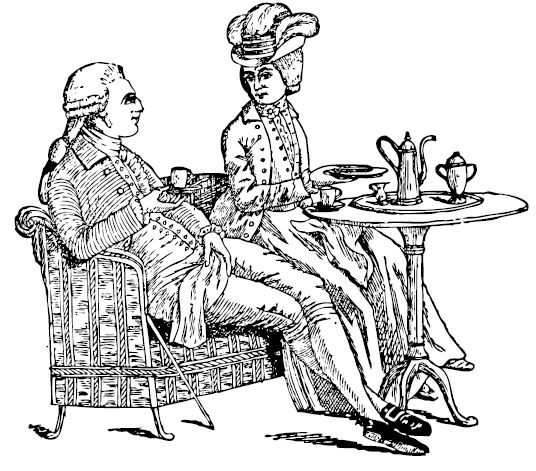
\includegraphics[width=0.8\textwidth]{paripoydassa.jpg}
\end{figure*}
\subsection*{Hileitä ja glitteriä}

\subsubsection*{DTM}
\textit{Mannerheimintie 6 B}

Luultavasti Suomen tunnetuin homo\-yökerho.
Vaikka DTM on tunnettu homobaarina,
ovat heterot myös löytäneet tiensä
Helsingin parhaimpaan tanssimestaan. Musiikki
on sen hetken hittibiisejä höystettynä
Kylie Minougella ja Gloria Gaynorilla.
\subsubsection*{Rymy-Eetu}
\textit{Erottajankatu 15--17}

Todella erilaista ja hauskaa paikkaa etsiessäsi:
Rymy-Eetussa on Octoberfest joka
päivä. Saksalaistyylisestä baariravintolasta
saa aamiaista yhdestätoista iltakuuteen asti
suhteellisen halvalla, ja tarjoilijatytötkin
ovat pukeutuneet saksalaistyylisiin asuihin.
Ruoka rehellistä ja rasvaista. Olutta
saa jopa litran tuopeissa ja kävijöitä kannustetaan
tanssimaan pöydillä -- meno
onkin tavallista baaria railakkaampaa ja
vapaampaa. Asiakaskunta on keskimäärin
keski-ikäisiä ja nuoria, ja musiikista huolehtii
illoittain vaihteleva live-bändi soittaen
humppaa ja ikivihreitä.
\subsubsection*{Kokomo}
\textit{Uudenmaankatu 16--20}

Helsingin ainut tikibaari vie sinut polynesialaistunnelmaan.
Tarjolla eksoottista
ruokaa sekä monipuolisesti erilaisia drinkkejä.
\subsection*{NPG-ravintolat}
Opiskelijat bilettävät nykyään paljon
aikaisempaa enemmän baareissa, ja järjestelypaikoista
kärjessä ovat Sedu Koskisen
entiset SK-ravintolat, nykyinen NPG. Ensimmäinen
asia, joka kannattaa muistaa,
varsinkin jos käy baareissa muutenkin kuin
opiskelijabileissä, membercardin hankkiminen.
Mainostusta tai ei, muutama ilmainen
parituntinen sekä euron tuopit tuovat
kortin hinnan äkkiä takaisin.
\subsubsection*{Apollo}
\textit{Mannerheimintie 16}

Forumin vanhan elokuvateatterin tiloihin avattu musiikkiclub, jossa on myös roast-keikkoja ja stand-upia.
\subsubsection*{Baarikärpänen}
\textit{Pohjoinen Rautatiekatu 21}

Bäkkärin ja Herkun kanssa samassa rakennuksessa sijaitseva Baarikärpänen on rento teiniyökerho, josta voi koulujen päättymisaikoina bongailla Tikkurilan lukiolaisia. Jos saapuu paikalle ennen yhtätoista, saa After Dark "-rannekkeen, jolla nauttii loppuillan juomat alennuksella.
\subsubsection*{Bar Bäkkäri}
\textit{Pohjoinen Rautatiekatu 21}

Ehdotonta rokkibaarien kärkeä. Keväällä~2016 hevibaari PRKL Club yhdisti voimansa Bäkkärin kanssa. Livemusaa viikoittain.
\subsubsection*{Club Capital}
\textit{Fredrikinkatu 51}

Tiger-niminen yökerho jaettiin kahtia vuonna~2013, ja glitterbileet jatkuvat nyttemmin Capitalissa. Helsingin suurin tanssilattia ja useampi baaritiski.
\subsubsection*{Kaivohuone}
\textit{Iso Puistotie 1}

Legendaarinen vuonna~1838 valmistunut huvila, joka muuttuu iltaisin tunnelmalliseksi yökerhoksi. Muista \\Limeksen Ex~Tempore "-bileet 3.9.2018 klo~21--!
\begin{figure*}[!b]
	\centering
	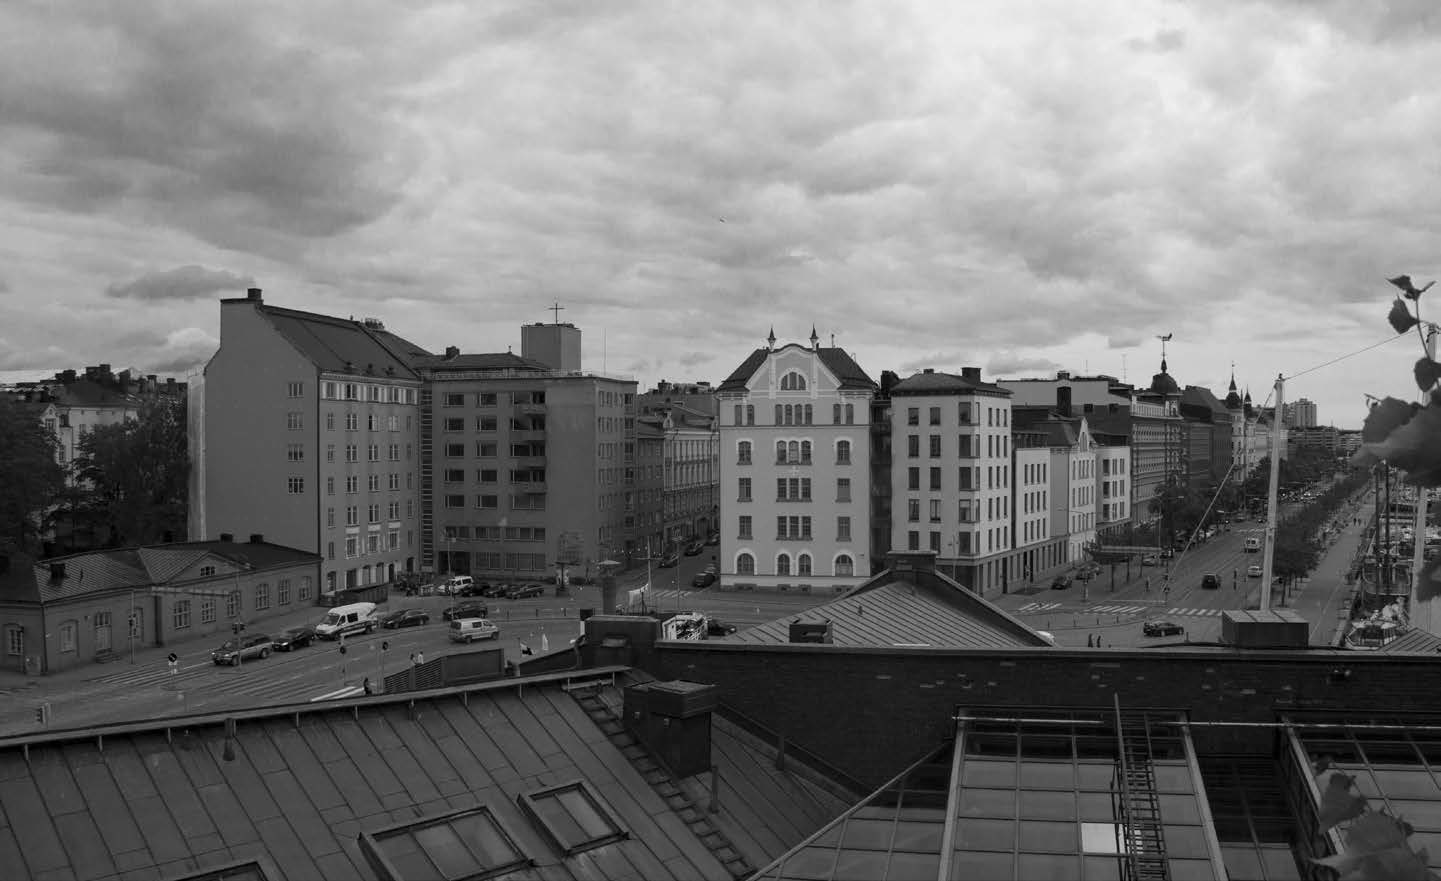
\includegraphics[width=\textwidth]{kadunnurkka.png}
\end{figure*}

\onecolumn
\section{Quo vadis?} {\small \itshape ``Minne matka ja millä?''}\vspace{0.5cm}

Oppaamme neuvoo sinulle reitit ja linjat kampusalueille sekä muihin tärkeisiin paikkoihin.
Lataa matkakortti ja ei kun menoksi! Tarkempia ohjeita: \url{www.reittiopas.fi}
\begin{figure}[!b]
	\centering
	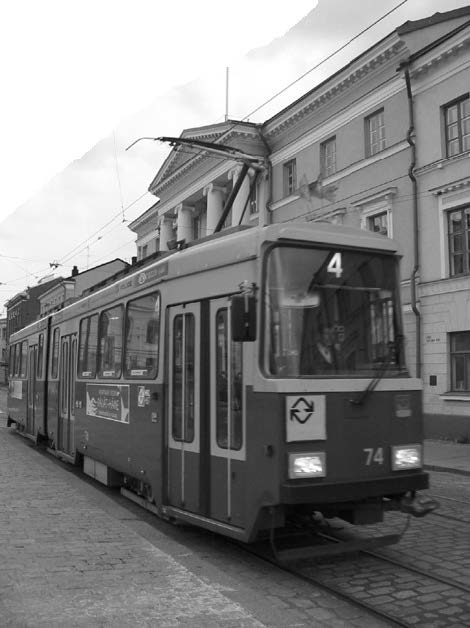
\includegraphics[width=0.6\textwidth]{nelosratikka.png}
\end{figure}
\subsection*{Kohteena Kumpula}
Raitiovaunu: 6, 8 \\
Sisäiset: 506, 52, 55, 56, 70, 71, 73, 74, 75, 77, 78 ja 79N \\
Seutuliikenne: 717, 718, 722, 724, 731, 738, 739, 765, 785--788
\subsection*{Tie vie Viikkiin}
Bussit: 506, 70, 71, 73, 74, 75, 77, 78 ja 79N\\
Seutuliikenne: 717, 718, 722, 724, 731, 738, 739, 765, 785--788
\subsection*{Otaniemi -- sielunkumppanit kutsuvat?}
Bussilla Sörnäiseen ja vaihto metroon.
\newpage
\begin{figure*}[!t]
	\centering
	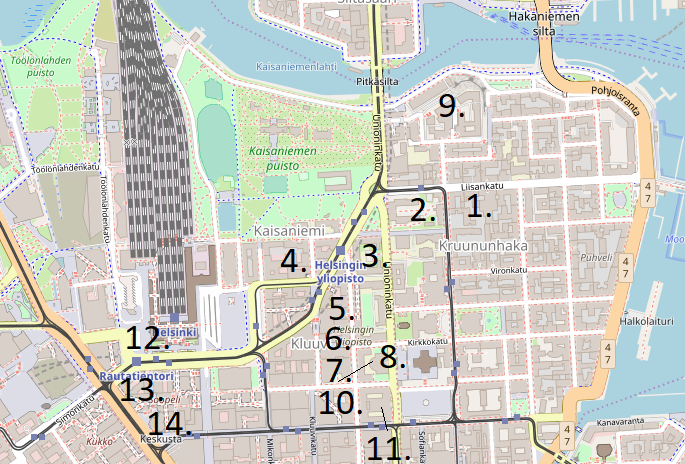
\includegraphics[width=0.8\textwidth]{keskustakartta.JPG}
	\caption{\textcopyright~OpenStreetMapin tekijät, lisätietoja osoitteista www.openstreetmap.org ja opendatacommons.org}
\end{figure*}
\begin{enumerate}
\item Limeksen entinen toimisto -- Liisankatu 16 D sisäpiha
\item Valtsika -- Unioninkatu 37
\item Metsätalo -- Unioninkatu 40
\item Avoin yliopisto -- Vuorikatu 20
\item Kaisa-kirjasto -- Vuorikatu 7
\item Aleksandria -- Fabianinkatu 28
\item Kielikeskus -- Fabianinkatu 26
\item Porthania -- Yliopistonkatu 3
\item Psykologia ja kasvatustieteet -- Siltavuorenpenger 20
\item Hallintorakennus; Unisportin liikuntatilat -- Yliopistonkatu 4
\item Päärakennus; mm.\,opiskelijaneuvonta -- Fabianinkatu 33
\item Yhteislähdöt saunailtoihin usein täältä -- Elielinaukio
\item Uusi ylioppilastalo; HYYn keskustoimisto, Alina-sali, osakunta- ja järjestötiloja --  Mannerheimintie~5
\item Vanha ylioppilastalo; Kuppila, Ylioppilasteatteri -- Mannerheimintie 3
\end{enumerate}

\newpage
\begin{figure*}[!t]
	\centering
	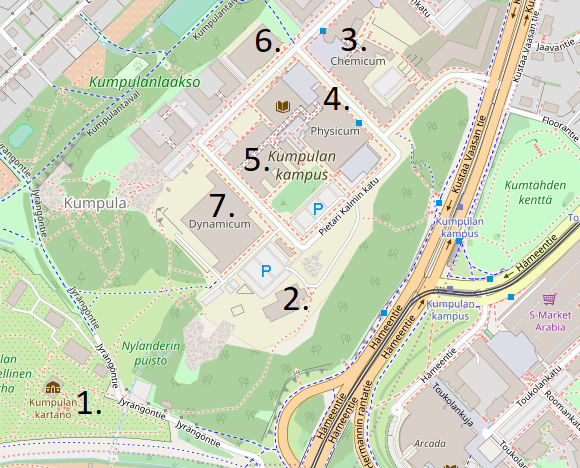
\includegraphics[width=\textwidth]{kumpulakartta.png}
	\caption{\textcopyright~OpenStreetMapin tekijät, lisätietoja osoitteista www.openstreetmap.org ja opendatacommons.org}
\end{figure*}
\begin{enumerate}
\item Kumpulan kartano, entinen MLTDK:n kanslia -- Jyrängöntie 2
\item Kiihdytinlaboratorio -- Pietari Kalmin katu 2
\item Chemicum -- A.I. Virtasen aukio 1
\item Physicum -- Gustav Hällströmin katu 2
\item Exactum -- Gustav Hällströmin katu 2b
\item Kumpulan liikuntahalli -- Väinö Auerin katu 11
\item Dynamicum -- Erik Palménin aukio 1
\end{enumerate}
\clearpage
\subsection*{Domus Academica ja Domus Gaudium}
Opiskelija-asuntojen lisäksi Leppäsuonkadulla
sijaisevalta Dommalta löytyy myös
uusi ylioppilastalo Domus Gaudium eli
Ilon Talo. Itse kukin vääntäköön siitä sitten
vitsiä\dots Ilon Talossa sijaitsee myös rakas
Klusterimme sekä erilaisia sauna- ja kokoustiloja.
\begin{figure*}[h!]
	\centering
	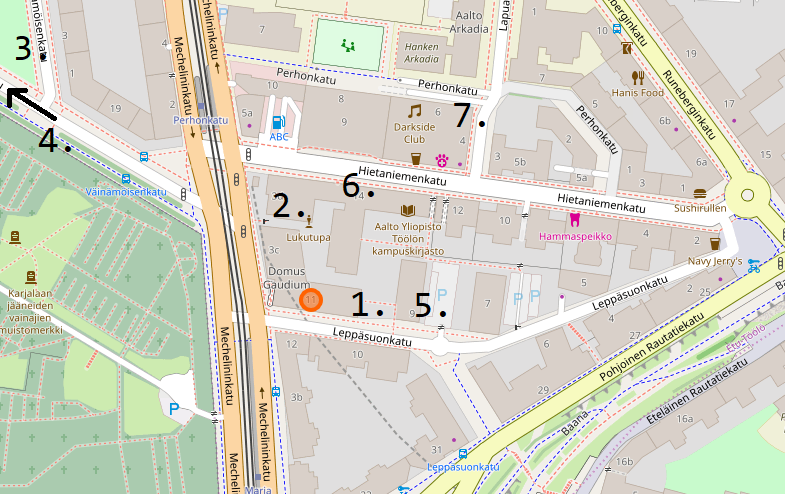
\includegraphics[width=0.8\textwidth]{dgkartta.png}
	\caption{\textcopyright~OpenStreetMapin tekijät, lisätietoja osoitteista www.openstreetmap.org ja opendatacommons.org}
\end{figure*}
\begin{enumerate}
	\item Matlu-klusteri ja kattosauna Sivistys -- Leppäsuonkatu 11
	\item Mechelininkadun Hub -- Mechelininkadu 3~D
	\item Väinämöisen puisto
	\item Hietsun ranta 
	\item Domma, A- ja B-talot -- Leppäsuonkatu 9
	\item Domus Academican C- ja D-talot -- Hietaniemenkatu 14
	\item Keskisuomalainen osakunta (Casa Academica) -- Perhonkatu 6
\end{enumerate}
\twocolumn

\section{Kun Stadi kyllästyttää\dots} {\small \itshape ``Liftausvinkkejä Helsingistä''}\vspace{0.5cm}

Mitä olisi Älä Hätäile "-opas ilman liftausvinkkejä?
Jos rahat ovat vähissä mutta
liikkeelle pitää päästä, liftaaminen on hauska
ja ilmainen etenemismuoto. Siistinnäköinen
ihminen tai pariskunta saa yleensä
Suomessa kyydin alle puolessa tunnissa,
mutta parinkin tunnin odotuksia sattuu
joskus kohdalle. Kannattaa varautua juotavalla,
eväillä, ylimääräisillä vaatteilla ja
sateensuojalla. Tiekartta auttaa kummasti.

Hyvä liftauspaikka on sellainen jossa
kuskit näkevät sinut hyvissä ajoin, ja jossa
on autolle tilaa pysähtyä. Kannattaa sijoittua
sopivan pysähtymisalueen, kuten bussipysäkin,
alkupäähän. Kun auto pysähtyy,
se yleensä ajaa 10--20~metriä ohi, jolloin
nappaat kassisi ja säntäät nopeasti kyydin
luokse. Moottoritiellä ei liftaaminen, eikä
käveleminenkään, ole sallittua. Poliisit tuskin
sakottavat mutta yleensä pyytävät poistumaan.

Ohimenevää liikennettä ei kannata
ajatella autoina vaan ihmisinä. Kun auto
lähestyy, pistä peukku pystyyn, näytä innokkaalta
ja iloiselta ja pyri saamaan katsekontakti
kuskiin. Ei aurinkolaseja, huppuja
tai syvälle painettuja hattuja. Voit myös
kehittää jostain kyltin. Liikkuvasta autosta
lukeminen
vaatii yllättävän suurta tekstiä:
A3 on parempi koko kuin A4. Kylttiin voit
kirjoittaa isolla ja selkeällä tekstillä määränpääsi,
tai seuraavan suuremman kaupungin nimen,
tai jotain muuta: Pois, Kauas, Merelle,
Kotiin.

\noindent Liftareita löytyy webistä: \url{hitchwiki.org}
\subsection*{Hankoon}
Moottoritie Länsiväylä kulkee koko Espoon
halki, emmekä tiedä onko yksikään
Länsiväylän liittymä hyvä liftauspaikka.
Emme myöskään ole kuulleet kenestäkään
joka olisi liftannut (paitsi yöllä baarista
kotiin) Ruoholahdessa juuri ennen Länsiväylän
alkua. Sen sijaan Espoon busseilla
voi mennä Länsiväylän loppupäähän Kivenlahteen/
Saunalahteen ja kävellä Espoonlahden
yli menevän sillan yli. Moottoritien
loputtua löytyy hyvä paikka.
\subsection*{Turkuun}
Turkuun on jostain syystä hiukan muita
suuntia heikommat yhteydet. Toimiva,
vaan ei täydellinen, paikka on Turun
moottoritien alku Munkkivuoressa. Huopalahdentien
(jolla motarin risteys on)
liikennevalot ja kaistajärjestelyt eivät ole
kovin suotuisia Huopalahdentien vierellä
liftaamiseen. Kannattaa ehkä mennä parikymmentä
metriä ramppia pitkin moottoritien
suuntaan: sieltä löytyy leveä kohta,
jossa autot voivat täysin turvallisesti poimia
liftarin kyytiin. Tosin todella huonolla
tuurilla sinipukuinen virkamies saattaa
käydä huomauttamassa, että paikka todella
on vasta vähän moottori\-tie\-liikenne\-merkin
jälkeen. Silloin voi palata takaisin Huopa\-lahden\-tielle
yrittämään. Toinen vaihtoehto
on kookas liittymä reilun kilsan Espoon
Keskuksesta pohjoiseen.
Sieltä kuulemma
löytyy liftauskelpoinen
ramppi, ja riittävästi
länteen menevää liikennettä.
\subsection*{Forssaan ja Poriin}
Pieni mukava Vihdintie Etelä-Haagan
liikenneympyrästä eteenpäin. Monet bussipysäkit
ovat hyviä liftauspaikkoja, mitä pidemmälle
menee bussilla, sitä vähemmän
paikallisliikennettä jää haaviin. Forssan
tai Humppilan kohdalla kääntymällä
tästä
saa myös vaihtoehtoisen reitin Turkuun tai
Tampereelle.
\subsection*{Hämeenlinnaan ja Tampereelle}
Ruskeasuolta, missä Mannerheimintie
muuttuu Hämeenlinnanväyläksi. Eka
bussipysäkki on hyvä, kuten myös seuraava,
SPR:n veripalvelun kohdalla oleva.
Myöhemminkin on hyviä paikkoja aina
Vantaalle ja Kehä III:lle asti. Esimerkiksi
Martinlaaksontien kohdalla, ja Keimolanportin
huoltoaseman kohdalla. Ennen Kehä
III:a Hämeenlinnanväylä ei ole moottoritie
(vaikka ehkä näyttääkin), joten liftaaminen
on täysin laillista. Koko matka Kehä III:lta
Tampereelle on sitten moottoritietä, joten
kannattaa varoa kyytejä, jotka jättäisivät
keskelle maaseutua johonkin hiljaiseen liittymään.
20~km ennen Hämeenlinnaa, Janakkalassa,
on (suoraan moottoritien päälle
rakennettu) suuri huoltoasemaravintolakompleksi
Linnatuuli. Se voi olla hyvä
paikka jäädä pois kyydistä, joka ei olisi
menossa enää paljoa pidemmälle, ja yrittää
saada uusi kyyti huoltikselta poistuvista
autoista.
\begin{figure}[!b]
	\centering
	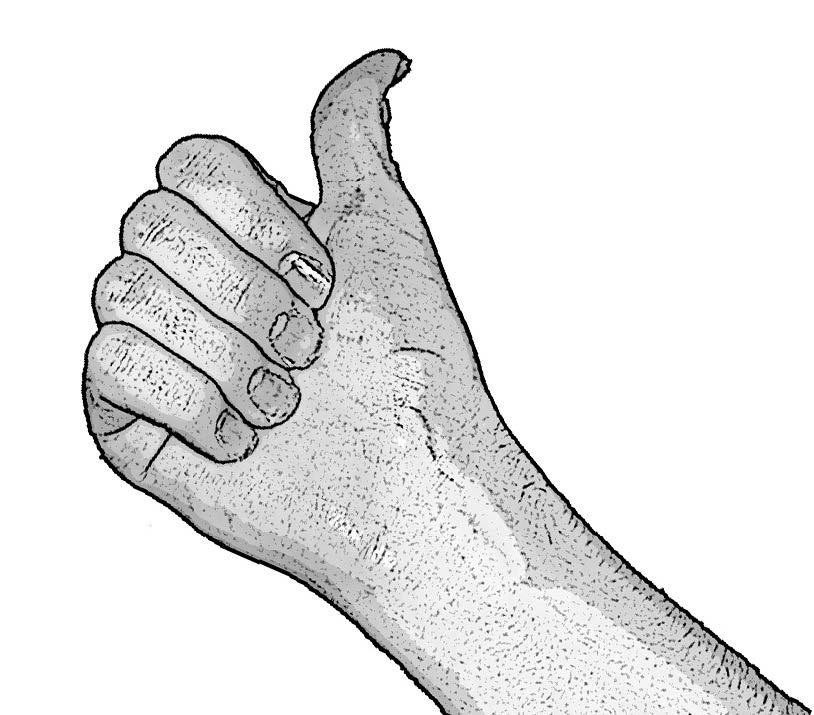
\includegraphics[width=\columnwidth]{liftauspeukalo.png}
\end{figure}
\subsection*{Lahteen}
Lahteen alkaa suora tie heti Kumpulan
kampuksen vierestä. Kampuksenkin bussipysäkki
on ihan OK liftipaikka niinä aikoina,
kun siihen ei koko ajan tule busseja.
Seuraava pysäkki on huono. Paras paikka
on kolmannen bussipysäkin (pysäkin nimi:
Valtimontie) jälkeinen pieni levike. (Moottoritie-
liikennemerkki on vähän inhasti
sijoitettu, mutta kyllä paikasta silti saa hyvin
kyytejä.) Osa tästä ajavista autoista on
menossa Porvooseen (ja Kouvolaan), joten
jos et halua sinne, kannattaa ennen kyytiin
nousua kysyä ja varmistaa, että kyyti on todella
menossa Lahteen päin. Koko matka
Lahteen on moottoritietä, joten myös kyyti
johonkin lähelle (kuten Keravalle tai Järvenpäähän)
saattaa jättää sinut liftaamaan
rampilla jossain liikenteeltään hiljaisessa
liittymässä.
Tällöin voi siirtyä moottoritietä
rinnan kulkevan Vanhan Lahdentien varrelle
koettamaan onneaan.
\subsection*{Porvooseen ja muualle itään}
(vaikka Pietariin ja Vladivostokiin)
Joko edellä mainitusta Valtimontien
pysäkiltä kysymällä (tai kyltin kanssa), tai
Itäväylältä Itäkeskuksen jälkeisiltä bussipysäkeiltä.
Parasta ehkä pyrkiä bussin~97
Mellunmäentien pysäkille asti, niin saa
suurimman osan paikallisliikenteestä pudotettua
haavin ulkopuolelle.

\twocolumn[\section{Frank} {\small \itshape ``Virtuaalinen kampus -- ja vähän päälle''}\vspace{0.5cm}]
Frank on korkeakoulu-, lukio-, ja ammattiopiskelijoiden
yhteinen opiskelijakortti (digitaalinen ja fyysinen),
joka otettiin käyttöön syksyllä~2013. Vaikka digitaalinen opiskelijakortti Frank App käykin jo kaikkialla Suomessa, voi fyysiseen opiskelijakorttiin yhdistää sähköavaimia tai kiinnittää ainejärjestöjen ja osakuntien jäsentarroja.

Frank on keskittynyt etenkin etujen tarjoamiseen,
ja etuja saa sekä myymälöissä
että myös nettikaupoissa, joista jälkimmäinen
vaati rekisteröitymisen netissä. Tämän
ohella opiskelijakortti toimii myös todistuksena, joka oikeuttaa opiskelijahintaiseen
ruokailuun UniCafeissa sekä
matkoihin Matkahuollossa (yli 80~km
matkoilla) ja VR:llä. Etuja voi tutkia
osoitteessa \url{https://student.frank.fi}.

Frankista on päätoimiselle
opiskelijalle saatavilla neljää eri
versiota: mobiili\-applikaatio Frank App, fyysinen opiskelijakortti maksu\-ominaisuudella tai ilman maksu\-ominaisuutta sekä
ISIC-yhdistelmä\-kortti,
joka tarjoaa maksuominaisuuden
ja Frankin tarjoaminen
etujen lisäksi
kansainvälisesti hyödynnettäviä
etuja.

Mobiiliapplikaatio Frank App maksaa \EUR{2,90}/12~kk. Maksuominaisuudella varustettu kortti on ilmainen 18--32-vuotiaille opiskelijoille, mutta samalla sitoudut Danske Bankin asiakkaaksi koko siksi ajaksi, kun haluat pitää kortin. Maksuominaisuudeton kortti maksaa \EUR{16,10}, ja sen kanssa saa myös digitaalisen opiskelijakortin lisenssin. Frank-ISIC "-kortista joutuu
maksamaan~\EUR{16} enemmän. ISIC-kortin kansainvälisyydestä voi olla kuitenkin monta mieltä, sillä Unkarista sillä ei ainakaan saanut opiskelija-alennuksia, vaikka tavallinen suomalainen opiskelijakortti olisi kelvannut.

Frank-kortin voi tilata menemällä osoitteeseen
\url{www.frank.fi/opiskelijakortti/} ja noudattamalla sivuilla olevia ohjeita. Muovinen opiskelijakortti täytyy varustaa vielä tiedekunnan kansliasta saatavalla lukuvuositarralla, jotta se kelpaa todistukseksi opiskelijastatuksesta. Frank App "-sovelluksen voi ladata App Storesta tai Google Playstä. 

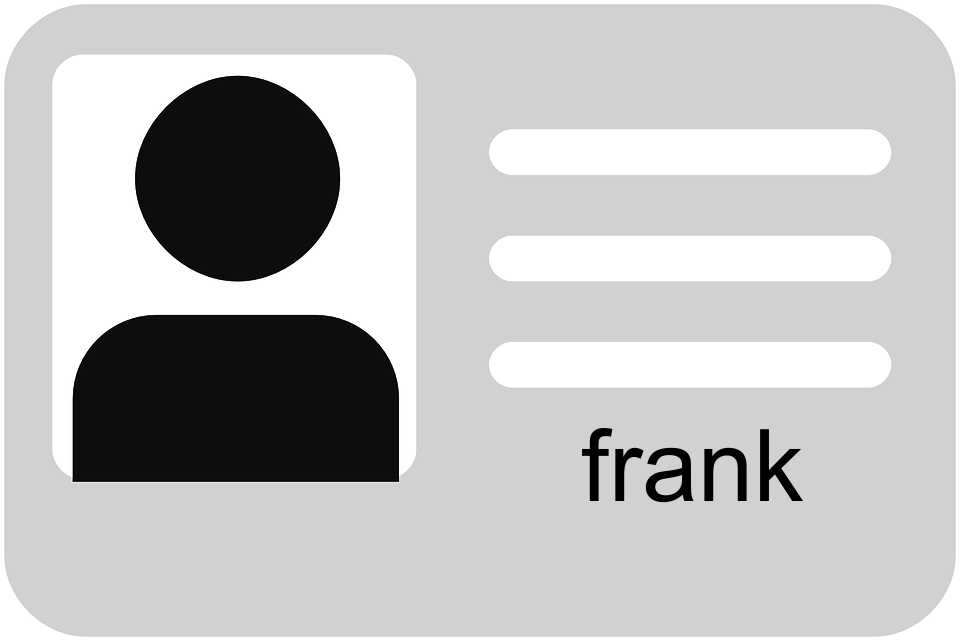
\includegraphics[width=\columnwidth]{card-158195_960_720.png}

\end{document}